%!TEX TS-program = knitr
\documentclass{article}\usepackage[]{graphicx}\usepackage[]{color}
%% maxwidth is the original width if it is less than linewidth
%% otherwise use linewidth (to make sure the graphics do not exceed the margin)
\makeatletter
\def\maxwidth{ %
  \ifdim\Gin@nat@width>\linewidth
    \linewidth
  \else
    \Gin@nat@width
  \fi
}
\makeatother

\definecolor{fgcolor}{rgb}{0.345, 0.345, 0.345}
\newcommand{\hlnum}[1]{\textcolor[rgb]{0.686,0.059,0.569}{#1}}%
\newcommand{\hlstr}[1]{\textcolor[rgb]{0.192,0.494,0.8}{#1}}%
\newcommand{\hlcom}[1]{\textcolor[rgb]{0.678,0.584,0.686}{\textit{#1}}}%
\newcommand{\hlopt}[1]{\textcolor[rgb]{0,0,0}{#1}}%
\newcommand{\hlstd}[1]{\textcolor[rgb]{0.345,0.345,0.345}{#1}}%
\newcommand{\hlkwa}[1]{\textcolor[rgb]{0.161,0.373,0.58}{\textbf{#1}}}%
\newcommand{\hlkwb}[1]{\textcolor[rgb]{0.69,0.353,0.396}{#1}}%
\newcommand{\hlkwc}[1]{\textcolor[rgb]{0.333,0.667,0.333}{#1}}%
\newcommand{\hlkwd}[1]{\textcolor[rgb]{0.737,0.353,0.396}{\textbf{#1}}}%

\usepackage{framed}
\makeatletter
\newenvironment{kframe}{%
 \def\at@end@of@kframe{}%
 \ifinner\ifhmode%
  \def\at@end@of@kframe{\end{minipage}}%
  \begin{minipage}{\columnwidth}%
 \fi\fi%
 \def\FrameCommand##1{\hskip\@totalleftmargin \hskip-\fboxsep
 \colorbox{shadecolor}{##1}\hskip-\fboxsep
     % There is no \\@totalrightmargin, so:
     \hskip-\linewidth \hskip-\@totalleftmargin \hskip\columnwidth}%
 \MakeFramed {\advance\hsize-\width
   \@totalleftmargin\z@ \linewidth\hsize
   \@setminipage}}%
 {\par\unskip\endMakeFramed%
 \at@end@of@kframe}
\makeatother

\definecolor{shadecolor}{rgb}{.97, .97, .97}
\definecolor{messagecolor}{rgb}{0, 0, 0}
\definecolor{warningcolor}{rgb}{1, 0, 1}
\definecolor{errorcolor}{rgb}{1, 0, 0}
\newenvironment{knitrout}{}{} % an empty environment to be redefined in TeX

\usepackage{alltt}

\usepackage[top=0.7in,bottom=1in,left=1in,right=1in]{geometry}
\usepackage{amsmath}
\usepackage{amssymb} % \mathbb
\usepackage[dvipsnames]{xcolor}
\usepackage{subcaption}
\usepackage{hyperref} % better ref than only url. 
\usepackage{ulem}
\usepackage{indentfirst} % indent the 1st paragraph
\usepackage[authoryear,round,comma]{natbib}
\usepackage{authblk} % make the title with multi authors
\usepackage{multirow} % table merge cubes
\usepackage{natbib}
\usepackage[titletoc,title]{appendix}
%\usepackage{arydshln}

\bibliographystyle{apa} 
            
\newcommand{\MYhref}[3][blue]{\href{#2}{\color{#1}{#3}}}%
\IfFileExists{upquote.sty}{\usepackage{upquote}}{}
\begin{document}
%\SweaveOpts{concordance=TRUE}

\title{A Functional Data Analysis Registration Model and Its Application to CO$_2$ Flux Data}

\author[1]{Fang He}
\author[2]{Duncan Murdoch}
\author[2]{Reg Kulperger}
\affil[1,2]{Department of Statistical and Actuarial Sciences, University of Western Ontario}
 
\maketitle


\textbf{Abstract.}  Carbon dioxide (CO$_2$) flux is needed for assessing and monitoring the annual carbon cycle. Only a small proportion of the land is currently covered by proper equipment to directly collect CO$_2$ flux data. With the help of the \underline{Mod}erate Resolution \underline{I}maging \underline{S}pectroradiometer (MODIS) which is carried by NASA satellites, corresponding data, such as normalized difference vegetation index (NDVI), is freely available from NASA. Our goal is building a model using MODIS data to predict the CO$_2$ flux data at any location. The CO$_2$ flux data has an obvious annual cycle with the phase changing from year to year. How to build a model to estimate the annual effect and seasonal dynamics is a challenging task. We use two models to analyze the data. The first model analyzes the data as a time series indexed by day, with additional covariates, such as species and NDVI. We use a  generalized additive model (GAM). One defect of this model is its inability to capture the seasonal dynamics. In the second model we treat each year as an independent multivariate observation. We use functional data analysis (FDA) to smooth the CO$_2$ flux data for each year separately. Then we use the FDA registration to standardize the seasonal dynamics. On the registered time scale, we build a model of the registered curves using a multivariate normal distribution. We use Dirichlet regression to model the seasonal dynamics and map the registered curves back to the natural time scale. These two steps allow us to simulate CO$_2$ flux on the natural time scale. We use 4 locations to conduct the study. The simulation results demonstrate the potential of the second model based on the FDA registration method.

\citep{marsrover}

\newpage

\tableofcontents

\newpage
 


\newpage

\section{Introduction}

Climate change has a big impact on plants and animal life. One thing that ecologists are interested in is phenology. i.e., the analysis of cyclic and seasonal natural phenomena, especially in relation to climate and plant and animal life. There are many ways to conduct the analysis. Current challenges include source data selection, gap filling techniques, and lack of comparison of current phenology study methods. There are usually two types of sources used in the phenology studies. One source is remote sensing data, the other is ground based data. Compared to the global wide remote sensing data, ground based data in a phenology study only covers a small portion of the land surface. Since it is costly to get ground based data at a new location, we are interested in building a model, and using remote sensing data to predict the ground based data.
 
How much carbon dioxide moves through a unit area per unit time is called carbon dioxide (CO$_2$) flux. 
CO$_2$ flux above-canopy/below-canopy measures the CO$_2$ consumption and production by plants.
CO$_2$ flux is an important component of the total atmospheric carbon balance, and it is important for the study of global climate change. 

Flux towers provide ground-based direct observations of carbon exchange. The tower is installed at a fixed location on the Earth.  Each tower works locally. Currently there are over 650 tower sites in the world working together, and forming a network of regional networks. 
Based on where the CO$_2$ fluxes are measured, there are soil-surface CO$_2$ flux, below-canopy CO$_2$ flux, above-canopy CO$_2$ flux, etc. Figure \ref{Fig:fluxtowers} shows flux tower examples.

\begin{figure}[!ht]
    \centering
    \begin{subfigure}[ht]{0.43\textwidth}
        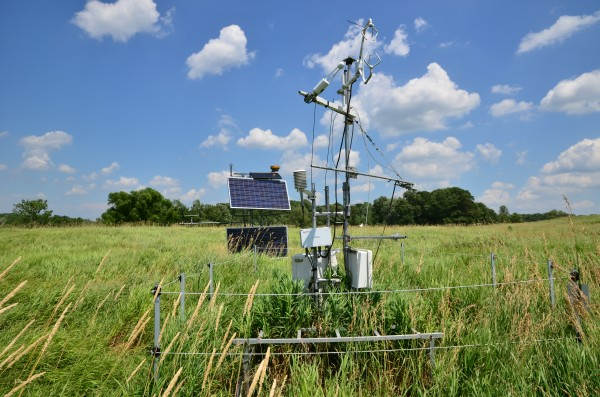
\includegraphics[width=\textwidth]{FluxTowerPic.jpg}
        \caption{Flux towers at MSU's Kellogg Biological Station. Photo credit: Bill Krasean.}
    \end{subfigure}
    ~ %add desired spacing between images, e. g. ~, \quad, \qquad, \hfill etc. 
      %(or a blank line to force the subfigure onto a new line)
    \begin{subfigure}[ht]{0.3\textwidth}
        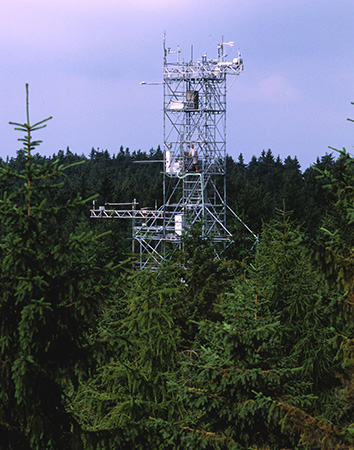
\includegraphics[width=\textwidth]{FluxTowerPic2.jpg}
        \caption{Flux tower that can measure below/above-canopy CO$_2$ flux.}
        \label{Fig:canopy}
    \end{subfigure}
        ~ %add desired spacing between images, e. g. ~, \quad, \qquad, \hfill etc. 
      %(or a blank line to force the subfigure onto a new line)
    \caption{Flux tower examples.}\label{Fig:fluxtowers}
\end{figure}

\begin{figure}[!ht]
\begin{center}
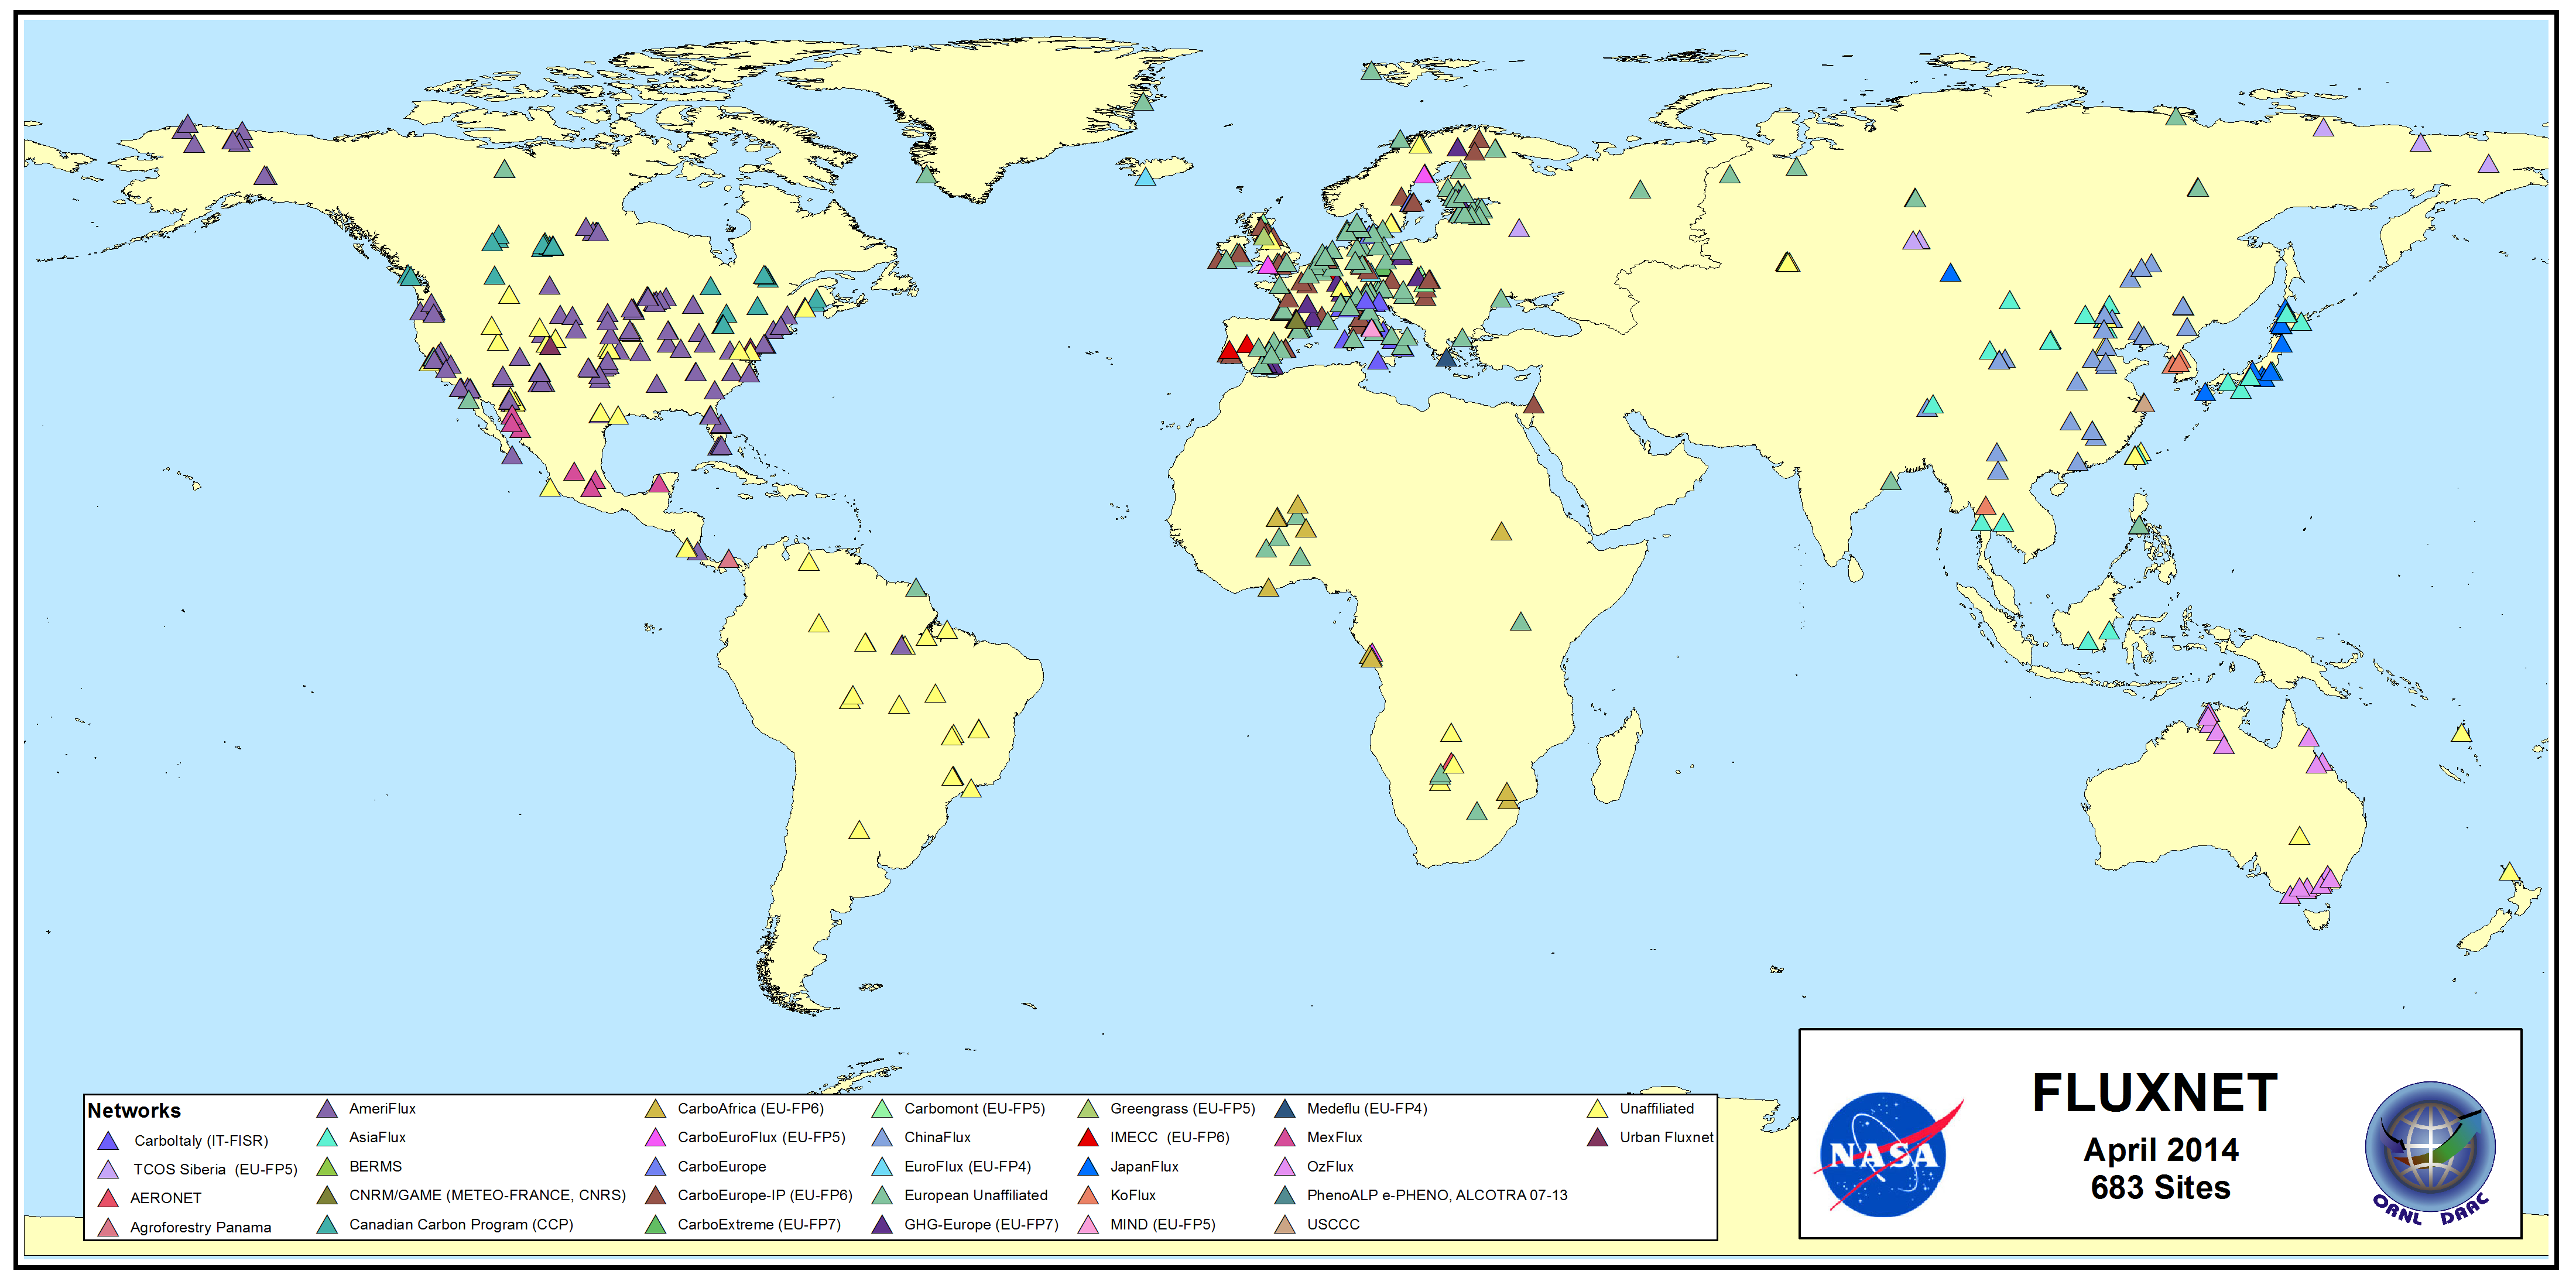
\includegraphics[width=13cm]{Fluxnet.png}
\caption{Distribution of flux tower networks. Photo credit: FLUXNET}
\label{Fig:Fluxnet}
\end{center}
\end{figure}

The distribution of the flux tower networks (Figure \ref{Fig:Fluxnet}) is not uniform.  A large proportion of the land is not covered by the flux tower network.  Between two adjacent flux towers, the flux is unknown. 

\smallskip

MODIS is the abbreviation for moderate-reslution imaging spectroradiometer.
The following information of MODIS is summarized from NASA website \url{http://modis.gsfc.nasa.gov/about/design.php}. MODIS is an instrument currently on board two satellites, Terra (December 1999) and Aqua (May 2002). It has 36 spectral bands, the wavelength is from 0.4$\mu$m to 14.4$\mu$m. The resolutions are 1 km or finer (2 bands at 250 m, 5 bands at 500 m, 29 bands at 1 km). The altitude of MODIS is 705 km.  It takes every 1 to 2 days for MODIS to scan the whole world.
 Figure \ref{Fig:MODIS} shows how MODIS works.

\begin{figure}[!ht]
    \centering
    \begin{subfigure}[ht]{0.3\textwidth}
        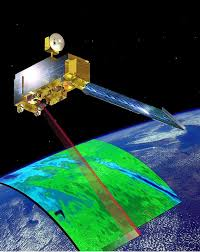
\includegraphics[width=\textwidth]{MODISpic2.jpeg}
        \caption{Photo credit: NASA}
    \end{subfigure}
    ~ %add desired spacing between images, e. g. ~, \quad, \qquad, \hfill etc. 
      %(or a blank line to force the subfigure onto a new line)
    \begin{subfigure}[ht]{0.37\textwidth}
        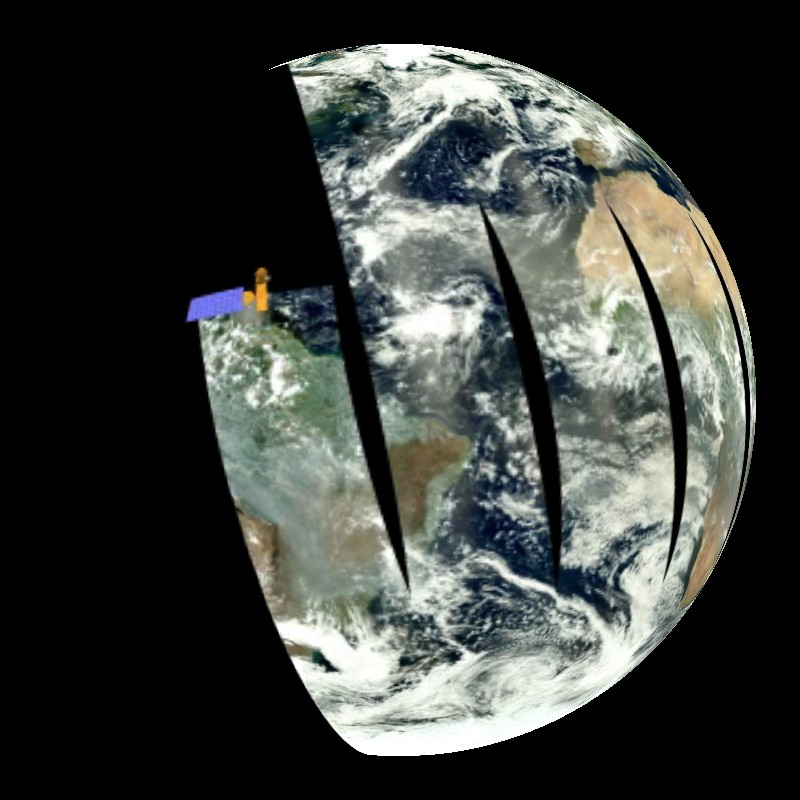
\includegraphics[width=\textwidth]{MODISpic1.jpg}
        \caption{Photo credit: NASA}
    \end{subfigure}
        ~ %add desired spacing between images, e. g. ~, \quad, \qquad, \hfill etc. 
      %(or a blank line to force the subfigure onto a new line)
    \caption{How MODIS works.}\label{Fig:MODIS}
\end{figure}

Four locations have been chosen in this study.
Each location collected above-canopy CO$_2$ flux data from ground stations and corresponding normalized difference vegetation index (NDVI) from MODIS. Figure \ref{Fig:NegCorr} shows negative dependency between the two measurements for each location. 

\begin{figure}[ht]
    \centering
    \begin{subfigure}[ht]{0.45\textwidth}
        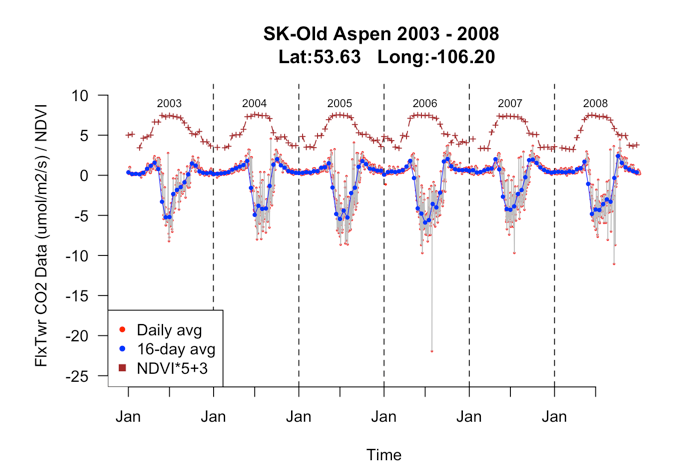
\includegraphics[width=\textwidth]{OAP_plot_together.png}
        \caption{Negative correlation between flux tower and MODIS data at SK-Old Aspen.}
        \label{Fig:NegCorr_OAP}
    \end{subfigure}
    ~ %add desired spacing between images, e. g. ~, \quad, \qquad, \hfill etc. 
      %(or a blank line to force the subfigure onto a new line)
    \begin{subfigure}[ht]{0.45\textwidth}
        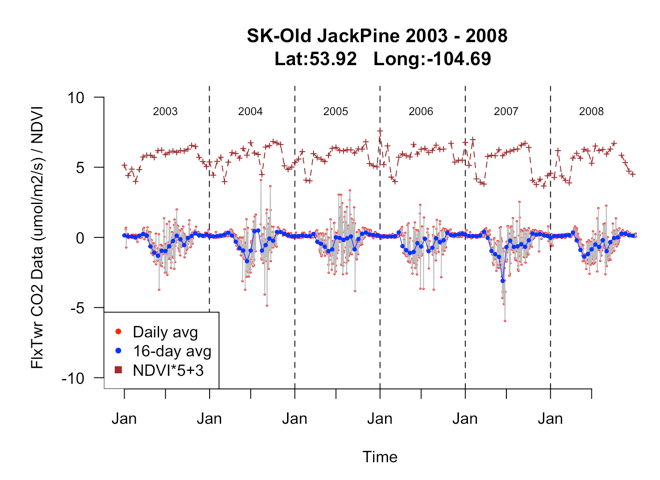
\includegraphics[width=\textwidth]{OJP_plot_together.png}
        \caption{Negative correlation between flux tower and MODIS data at SK-Old Jack Pine.}
        \label{Fig:NegCorr_OJP}
     \end{subfigure}
        ~ %add desired spacing between images, e. g. ~, \quad, \qquad, \hfill etc. 
      %(or a blank line to force the subfigure onto a new line)
      \begin{subfigure}[ht]{0.45\textwidth}
        \includegraphics[width=\textwidth]{SOU_plot_together.png}
        \caption{Negative correlation between flux tower and MODIS data at SK-Southern Old Black Spruce.}
        \label{Fig:NegCorr_SOU}
     \end{subfigure}
     ~
      \begin{subfigure}[ht]{0.45\textwidth}
        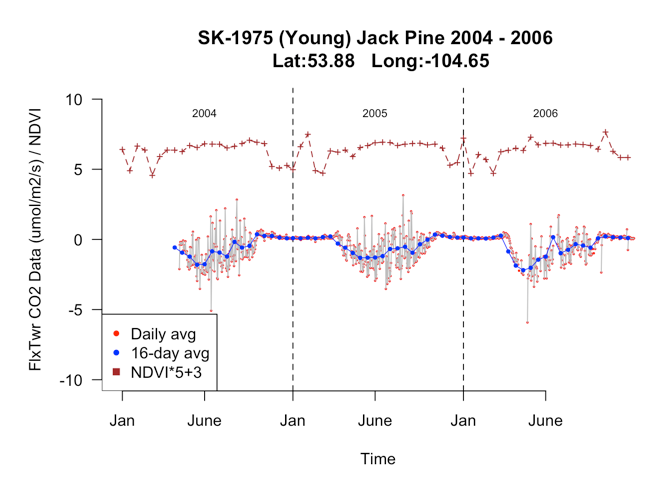
\includegraphics[width=\textwidth]{YJP_plot_together.png}
        \caption{Negative correlation between flux tower and MODIS data at SK-Young Jack Pine.}
        \label{Fig:NegCorr_YJP}
     \end{subfigure}
    \caption{Negative dependency between two measurements.}\label{Fig:NegCorr}
\end{figure}

NASA releases the  global data collected by MODIS,  such as NDVI,  leaf area index, temperature and emissivity, and thermal anomalies and fire, free of charge for the public.  Statistical models can be built combining both nearby CO$_2$ flux data and corresponding satellite data to predict the CO$_2$ flux data at a new location. With the help of proper statistical models, we can estimate the CO$_2$ flux at a wider area.

\smallskip

The following three chapters give the scientific background: 
 a brief introduction of MODIS and carbon dioxide flux appears in Section \ref{Sec:Background}, followed by relevant research that has been done by ecologists and statisticians (Section \ref{Sec:LiteratureReview}), and the display of the data we used in this proposal, including how flux data locations were selected and preprocessed (Section \ref{Sec:Data}).
We used two approaches to analyze our data. 
We describe our efforts to apply a class of additive models in Section \ref{Sec:AddModel}, followed by sections on using functional data analysis. 
Section \ref{Sec:SplineSmoothing} shows how we apply spline smoothing. Functional registration is described in Section \ref{Sec:Regi}. Section \ref{Sec:MultiNormal} and Section \ref{Sec:DiriReg} present  how we apply multivariate normal and Dirichlet regression to further simulate CO$_2$ flux data at a specific location.  
To simulate the CO$_2$ flux data at a wider range, one commonly used spatial model is Kriging. A brief introduction of Kriging presents in Section \ref{SubSec:Kriging}.
Section \ref{Sec:Conclusion} gives a short conclusion, and summarizes the model we proposed. 
We present the future work in Section \ref{Sec:FutureWork}.


\bigskip

\section{Background}\label{Sec:Background}

In the Introduction we mentioned two data types, CO$_2$ flux and MODIS data. In this section we will discuss them in more detail. 
Section \ref{SubSec:ModisData} will give a brief description of what NASA's Earth Observing System (EOS) is and the importance of having EOS. The relationship of EOS and Terra and Aqua will be shown. 
Section \ref{SubSec:FluxData} will present basic information about different types of CO$_2$ flux together with eddy covariance which is currently the standard method used by ecologists to measure fluxes of trace gases between ecosystems and the atmosphere. 

\subsection{MODIS Data}\label{SubSec:ModisData}

According to NASA's EOS project science office \url{http://eospso.nasa.gov/}  ``EOS is a coordinated series of polar-orbiting and low inclination satellites for long-term global observations of the land surface, biosphere, solid Earth, atmosphere, and oceans''. Figure \ref{Fig: NASA EOS} shows Terra and Aqua, two missions of EOS.  
\begin{figure}[!ht]
\begin{center}
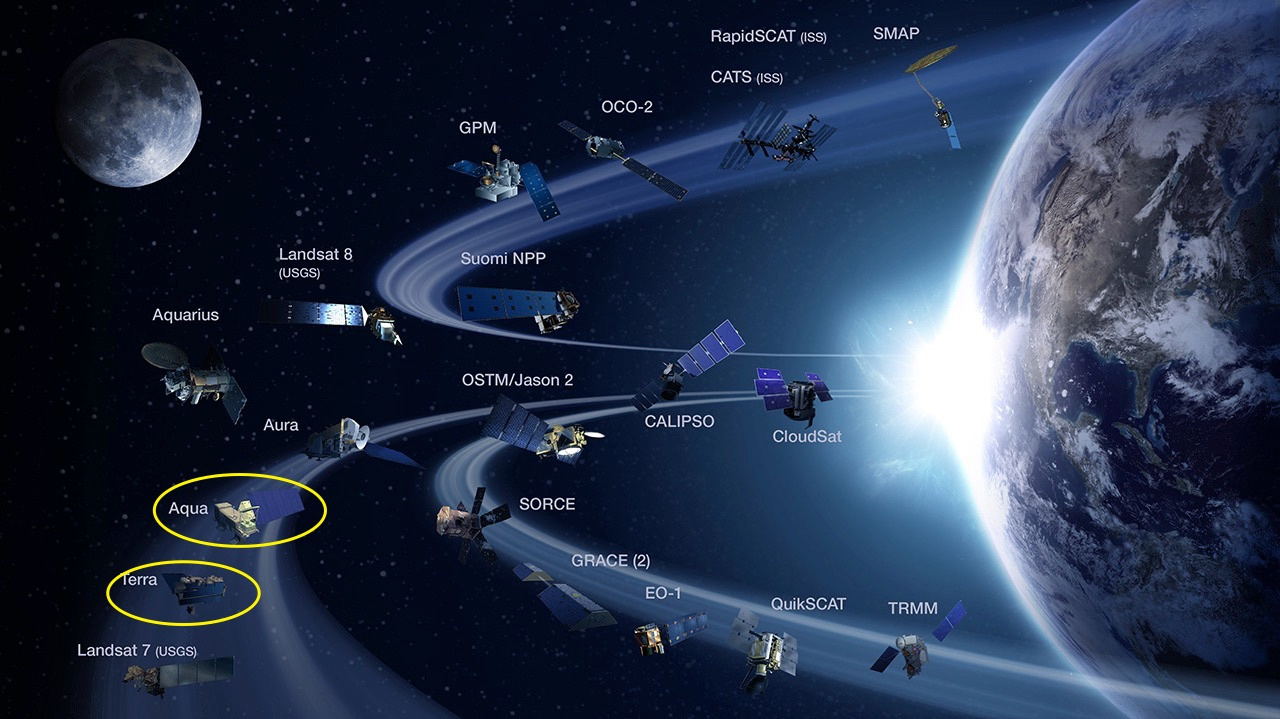
\includegraphics[width=16cm]{nasaEOS.png}
\caption{NASA Earth science division operating missions.}
\label{Fig: NASA EOS}
\end{center}
\end{figure}


Table \ref{Tab:TnA} is summarized from \url{http://science.nasa.gov/missions/terra/} and \url{http://atrain.nasa.gov/publications/Aqua.pdf}.

\begin{table}[!ht]
\caption{Some details of Terra and Aqua satellites}\label{Tab:TnA}
\centering
\def\arraystretch{1.5}
\begin{tabular}{c|cccc}
& \multirow{2}{*}{\textbf{Primary Mission}} &\multirow{2}{*}{\textbf{Lauched Day}} 
& \multicolumn{2}{c}{\textbf{Passes equator}}\\
\cline{4-5}
& & & \textbf{Direction} & \textbf{Time}\\
\hline
\textbf{Terra} & atmosphere, land, and oceans & Dec 18, 1999  & North to South & Morning\\
\textbf{Aqua} & water, radiative energy flux, aerosols, etc. & May 4, 2002  & South to North & Afternoon
\end{tabular}
\end{table}



\begin{figure}[!ht]
\begin{center}
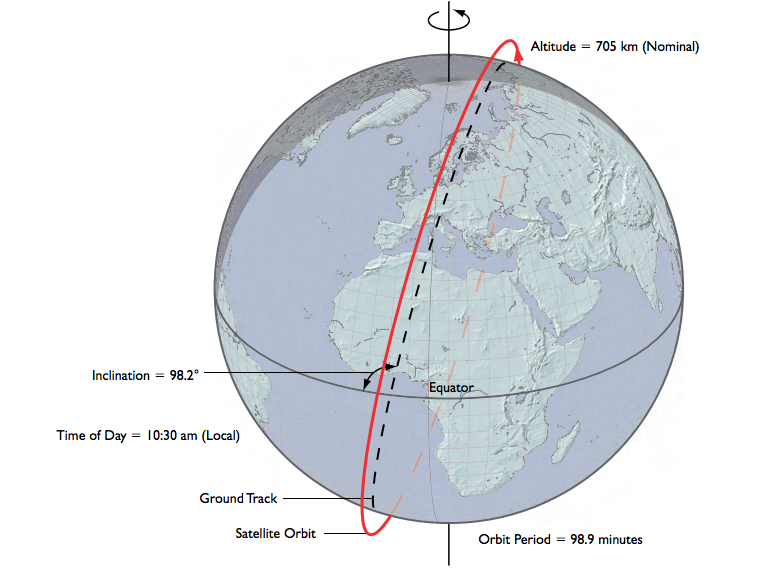
\includegraphics[width=12cm]{inclination.png}
\caption{3D model of Terra Satellite orbit.\citep{king2007our}}
\label{Fig: 3DTerra}
\end{center}
\end{figure}



Both satellites are in sun-synchronous orbits. The orbital plane rotates approximately one degree each day eastwards to keep pace with the Earth's movement around the sun. In this way, the satellite passes over any given point of the planet's surface at the same local solar time. The data can be transmitted directly from the spacecraft to ground stations equipped with an average 3m or larger X-band receiving system and appropriate hardware and software, though the raw data received from MODIS can not be used directly.  It needs decoding, interpretation, scaling, and positioning. NASA processes the raw MODIS data in different forms and stages known as products. Table \ref{Tab:modisproduct} shows definitions of MODIS products from level 0 to level 4.

\begin{table}[!ht]
\caption{Definitions of MODIS data processing levels.}\label{Tab:modisproduct}
\centering
\begin{tabular}{|c|c|}
\hline
Product Levels & Product Definitions\\
\hline
Level 0 & Unprocessed instrument data.\\
\hline
Level 1A & Unprocessed instrument data alongside ancillary information.\\
\hline
Level 1B & Data processed to sensor units, e.g. brightness temperatures.\\
\hline
Level 2 & Derived geophysical variables, e.g. sea ice concentration.\\
\hline
Level 3 & Variables that are mapped on a grid, e.g. data using EASE-Grid.\\
\hline
Level 4 & Modeled output or variables derived from multiple measurements.\\
\hline
\end{tabular}
\end{table}

MODIS data used in this thesis was collected from \MYhref[black]{http://daac.ornl.gov/MODIS/}{the Oak Ridge National Laboratory Distributed Active Archive Center (ORNL DAAC) MODIS land product subsets}.

\subsection{Carbon Dioxide Flux Data}\label{SubSec:FluxData}

Flux measurements are widely used to estimate the exchange of heat, water, and carbon dioxide, as well as methane and other trace gases. CO$_2$ flux is dependent on the amount of CO$_2$ crossing an area, the size of the area being crossed, and the time it takes to cross this area.

Due to the complicated ecosystems of forests, different functional properties can be characterized by distinctive layers \citep{misson2007partitioning}.
Based on the CO$_2$ flux measuring height, there are 3 different types CO$_2$ flux data. They are Soil CO$_2$ flux, CO$_2$ flux below-canopy, and CO$_2$ flux above-canopy.

\begin{figure}[!ht]
\centering
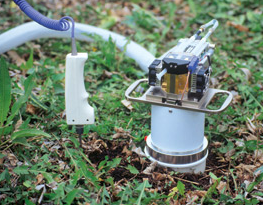
\includegraphics[width=6cm]{soilflux.png}
\caption{6400-09 Soil CO$_2$ flux chamber.}
\label{Fig:soilflux}
\end{figure}

Soil CO$_2$ flux measures a physical process driven primarily by the CO$_2$ concentration diffusion gradient between the upper soil layers and the atmosphere near the soil surface. Figure \ref{Fig:soilflux} shows a device measuring soil CO$_2$ flux. Figure \ref{Fig:canopy} is an example of how the below/above-canopy CO$_2$ flux gets measured.

The eddy covariance method is one of the most direct and defensible ways to measure such fluxes. The ``covariance'' in eddy covariance method is different from the definition of covariance in statistics. For more information, please see Appendix \ref{App:EddyCov}. Uniform terminology and single methodology are still being developed for the eddy covariance method.  Much of the effort is being done by network (e.g., FluxNet, ICOS, NEON, ect.)  to unify various approaches. FLUXNET, a ``network of regional networks'', coordinates regional and global analysis of observations from micro meteorological tower sites. One of the conventional ways to calculate vertical fluxes is

\begin{equation}
F = \overline{\rho_a\omega s},
\end{equation}
where $\omega$ denotes the vertical wind speed, $s$ represents the mixing ratio, the $\rho_a$ means air density, and the bar over the product of the three parameters means average.  

Flux tower data used in this thesis came from the Canadian Carbon Program (CCP).
Figure \ref{Fig:QCmodis} shows 8 years of CO$_2$ flux above-canopy data at Quebec City of harvested black spruce/jack pine. No obvious annual pattern showed up. The positive records of CO$_2$ flux occur during periods when the plants release more CO$_2$ than the amount they absorb, and records are negative when more CO$_2$ is absorbed by photosynthesis than is released by respiration.

\begin{figure}[!ht]
\centering
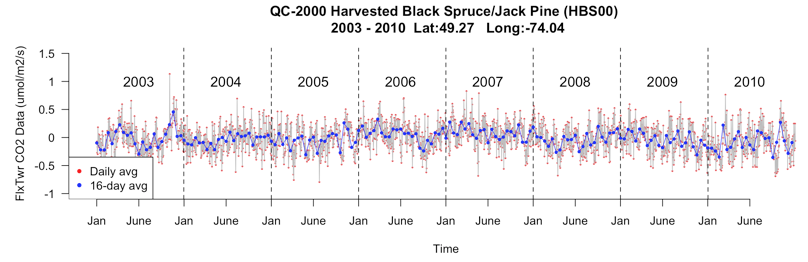
\includegraphics[width=14cm]{QCmodis1.png}
\caption{Quebec City harvested black spruce/jack pine CO$_2$ flux data from 2003 to 2010.}
\label{Fig:QCmodis}
\end{figure}

\section{Literature Review}\label{Sec:LiteratureReview}

There are 44 MODIS products (MOD01 -- MOD44) with different processing levels that can be used to study global climate change.
The flux tower networks also collect ground-based data over the years. 
Many studies have been done that use either the MODIS data or the flux tower data, or use MODIS and flux tower data together. 
\subsection{Ecology}

In ecology, many studies covered the following 3 topics.

1. Comparing the biomass calculated by MODIS and flux data separately. Biomass, such as regional evaporation and gross primary production (GPP) which is the amount of chemical energy produced in a given length of time are used in the studies. \citet{heinsch2006evaluation} and \citet{kalfas2011modeling} described studies about calculating GPP from MODIS and flux data, and revealing the relationship of the estimations by linear regression. Similar analysis has been applied to evaporation \citep{cleugh2007regional}.


2. Since the data collection of MODIS and flux tower are highly dependent on weather conditions, together with unexpected mechanical defects, gap filling techniques were  developed. \citet{moffat2007comprehensive} showed comparisons of gap filling techniques for carbon flux data.

3. Using both MODIS data and flux data to study the phenology. \citet{klosterman2014evaluating} discussed using 3 different sigmoid functions to estimate phenology dates, and comparing the data driven outcomes with visual assessment.  The challenges as summarized in \citet{klosterman2014evaluating} in the current study of phenology include lacking standard protocols of choosing proper biological events, lacking comparisons of current methods of transition dates estimation (e.g. the start of spring, the end of fall).

The studies using MODIS and flux data cover a variety of aspects. Besides the above three topics, machine learning techniques are used in the prediction of GPP \citep{yang2007developing} and evapotranspiration \citep{yang2006prediction}.  A continental scale model was built by support vector machine (SVM).   

\subsection{Statistics}

In statistics, functional data analysis is one of the appropriate tools to analyze the underlying patterns of our data. 
One assumption of FDA is that the underlying process generating the data is smooth.
\citet{levitin2007introduction} mentioned ``FDA was designed to take advantage of replications''.
``The primary advantage of FDA is that it allows the researcher to ask questions about when in a time series diffferences may exist between two or more sets of observations." \citep{levitin2007introduction}

A functional datum is not a single observation but a set of measurements over a continuum, usually time.
A typical analysis of functional data begins with using smoothing techniques to represent each observation as a functional object. The original data are then set aside, and the smooth estimated curves are used for further analysis. 

Application of FDA has appeared in a large number of publications across multiple fields, such as medicine, chemistry, managerial science, and ecology.
Medical research including shape analysis and gene information extraction. 
\citet{epifanio2011functional,epifanio2014hippocampal} published their analysis of applying FDA in bone shape and hippocampal shape analysis by using registration tools and functional principle component analysis (fPCA). Besides shape analysis, \citet{leng2006classification} and \citet{reimherr2014functional} applied FDA in gene and genetic association studies. \citet{tian2010functional} mentioned functional data analysis in brain imaging studies. 
\citet{burfield2015review} introduced the application of FDA in chemical data. 
\citet{dass2012introducing} and \citet{muelas2016facing} gave application of FDA in business. \citet{gorrostieta2014characterization} and \citet{martinez2014air} described the application of FDA in ecology. 


\citet{martinez2014air}, \citet{reimherr2014functional}, and \citet{nikitovic2011functional} not only used FDA in the analysis, but compared the results with traditional multivariate methods as well.

\begin{figure}[!ht]
\centering
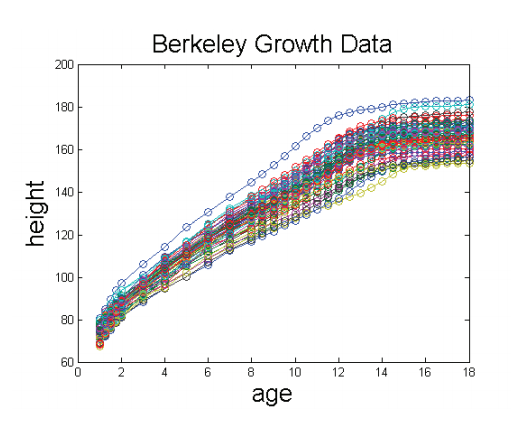
\includegraphics[width=8cm]{egsmooth.png}
\caption{Functional data smoothing example. \citep{FDAGiles}}
\label{Fig:fdasmooth}
\end{figure}

Figure \ref{Fig:fdasmooth} is an example of functional data smoothing. Heights of 20 girls were taken from ages 0 through 18 with unevenly spaced time points. The circles in Figure \ref{Fig:fdasmooth} represent the original data points. The smooth lines are the fitted curves for each girl.
\citet{ramsay2006functional} also mentioned the first steps in a functional data analysis are smoothing and interpolation. 
After functional data smoothing, we can estimate the height of a given girl at any age between 0 and 18. One of the advantages of functional data smoothing is that we can get continuous derivatives. The second derivatives of Figure \ref{Fig:fdasmooth} are shown in the left panel of Figure \ref{Fig:fdaregi}.

The individual differences of height acceleration curves makes the overall pattern not so obvious. It makes more sense that we compare ``the pubertal growth spurts of two children at their respective ages of peak velocity rather than at any fixed age'' \citep{ramsay2006functional}. The feature alignment technique is called functional data registration. Figure \ref{Fig:fdaregi} compares the original data with the data after registration.

\begin{figure}[!ht]
\centering
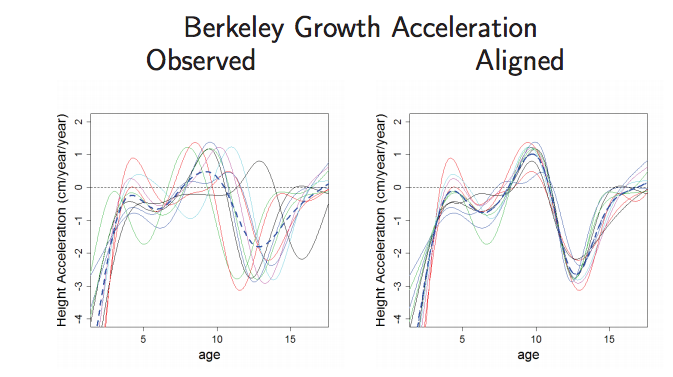
\includegraphics[width=14cm]{egregistration.png}
\caption{Functional data registration example. \citep{FDAGiles}}
\label{Fig:fdaregi}
\end{figure}

One way to conduct registration is landmark registration. 
A landmark or a feature of a curve is some characteristic that one can associate with a specific argument value. Landmarks are typically maxima, minima, or zero crossings of curves.
They may be identified with zeros at the level of some derivatives.

The landmarks chosen in our study are bounded and ordered between 0 and 365, they are all positive and dependent with each other. The Dirichlet regression \citep{hijazi2009modelling} turned out to be an appropriate tool to model their behaviour. Dirichlet regression always applies to compositional data (positive proportions sum up to one). Compositional data are used in chemistry  and related fields.  \citet{gueorguieva2008dirichlet} applied Dirichlet regression to psychiatric data.  \citet{maier2014dirichletreg} showed examples of how to use R to conduct Dirichlet regression. \citet{boukal2015analyses} introduced the application of Dirichlet regression in developmental rate isomorphy in ectotherms. 


\section{Data}\label{Sec:Data}

The NDVI data we downloaded from ORNL DAAC MODIS land product subsets is level 3, 16-day average data. The quality of MODIS data is highly sensitive to the visibility of the day. The 16-day average data does not exactly take the average over 16 days of data, but may choose the most desirable record among the 16 day collections to represent it. 
The frequency of CO$_2$ flux above-canopy collected from CCP is every 30 minutes. For two different types of data, having the same frequency will be easier for later analysis. We took the daily average of CO$_2$ flux above-canopy data first. Then we took the 16 day average of the daily average of CO$_2$ flux above-canopy data. Since 365 is not a multiple of 16, the first 22 16-day average CO$_2$ flux above-canopy data were each calculated by 16 daily average CO$_2$ flux above-canopy data, while the last 16-day average data was calculated by only 13 daily average data. Figures \ref{Fig:OAPmodis} to \ref{Fig:YJPmodis} show the plots of daily average and 16-day average of CO$_2$ flux above-canopy data together for 4 different locations.

\subsection{Location Selection}

Flux towers give researchers the ability to watch as carbon dioxide concentrations vary between the earth and atmosphere, signalling the increase or decrease of the gas.
There are 32 sites in the CCP. We wanted our CO$_2$ flux above-canopy data to meet the following requirements.

\begin{enumerate}
\item Each site has at least 3 years high quality CO$_2$ flux above-canopy data showing an annual pattern.
\item Sites are geometrically close to each other.
\item Each site has only one species, but we want multiple species over the selected sites.
\end{enumerate}

We checked the data at 32 CCP sites one by one.

\begin{table}[!ht]
\centering
\caption{18 sites that have CO$_2$ flux above-canopy data.}
\label{Tab:havedata}
\begin{tabular}{|c|c|}
\hline
Site Name & Data Collection Timeframe  \\
\hline
BC-Campbell River 1949 Douglas-fir & 1997-2015  \\
BC-Campbell River 1988 Douglas-fir & 2001-2015  \\
BC-Campbell River 2000 Douglas-fir & 2000-2015  \\
\hline
NB-Charlie Lake 1 1975 Balsam fir & 2003-2005  \\
\hline
ON-Borden Mixedwood & 1995-2015  \\
ON-Groundhog River Mixedwood & 2003-2015  \\
ON-Turkey Point 1939 White Pine & 2003-2015  \\
ON-Turkey Point 1974 White Pine & 2003-2015  \\
ON-Turkey Point 1989 White Pine & 2003-2015  \\
ON-Turkey Point Decidous & 2012-2014  \\
\hline
QC-2000 Harvested Black Spruce/Jack Pine (HBS00) & 2001-2010 \\
QC-Eastern Old Black Spruce (EOBS) & 2003-2010 \\
\hline
SK-1975 Young Jack Pine & 2003-2015\\
SK-2002 Jack Pine & 2003-2015 \\
SK-1994 Jack Pine & 2001-2015 \\
SK-Old Aspen & 1996-2015 \\
SK-Old Jack Pine &  1994-2015 \\
SK-Southern Old Black Spruce & 1994-2015\\
\hline
\end{tabular}
\end{table}

Table \ref{Tab:havedata} shows that 18 out of 32 sites recorded CO$_2$ flux above-canopy data. 
The time frame listed in Table \ref{Tab:havedata} is the data collecting time range of each site listed on CCP website. The actual time range of collecting CO$_2$ flux above-canopy data sometimes will be much shorter, and varies a lot from site to site. 

Data collected at BC-Campbell River area has only one species, Douglas fir. NB-Carlie Lake area did not provide enough data. ON-Turkey Point White Pine has no exact canopy height information listed on line. Mixed wood has more than one species, we will consider this more complicated data later.



When all of these rules were applied, we ended up with 4 sites of data as shown in Table \ref{Tab:FluxData}.

\begin{table}[!ht]
\caption{CO$_2$ flux above-canopy data information.}\label{Tab:FluxData}
\centering
\begin{tabular}{ccccc}
\hline
\textbf{Longitude} & \textbf{Latitude} & \textbf{Site Name} & \textbf{Time Range} & \textbf{Data Type}\\
\hline
-106.1978 & 53.6289 & SK Old Aspen & 2003 - 2008 & CO$_2$ Flux Above Canopy 39m\\
-104.6920 & 53.9163 & SK Old Jack Pine & 2003 - 2008 & CO$_2$ Flux Above Canopy 28m\\
-105.1178 & 53.9872 & Sk Southern Old Black Spruce & 2003 - 2008 & CO$_2$ Flux Above Canopy 25m\\
-104.6453 & 53.8758 & Sk 1975 (Young) Jack Pine & 2004 - 2006 & CO$_2$ Flux Above Canopy 16m\\
\hline
\end{tabular}
\end{table}

\subsection{Data View}

The 16-day average data of SK Old Aspen (Figure \ref{Fig:OAPmodis}) shows slightly increasing trend from January to April, slightly decreasing trend from October to December,and a sharp decreasing trend followed by a sharp increasing trend from April to October each year. There is one influential data point of the daily average in 2006.



\begin{figure}[!ht]
\centering
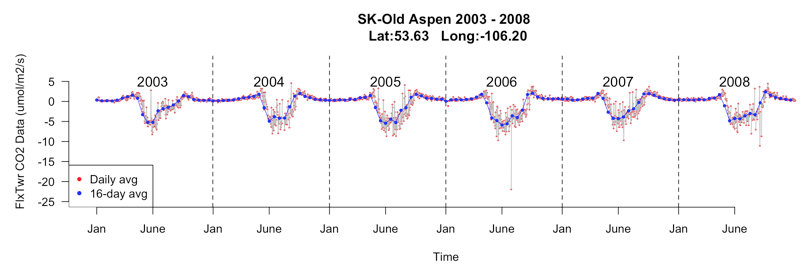
\includegraphics[width=14cm]{OAPmodis1.png}
\caption{Saskatchewan old aspen CO$_2$ flux data from 2003 to 2008.}
\label{Fig:OAPmodis}
\end{figure}


The 16-day average data of SK Old Jack Pine (Figure \ref{Fig:OJPmodis}) has narrower range of fluctuation, compared to SK Old Aspen. The underlying annual trend is not as obvious as SK Old Aspen.  There is an interesting W shaped pattern in 2004.




\begin{figure}[!ht]
\centering
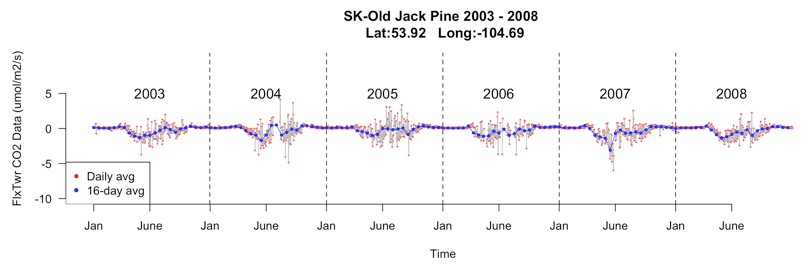
\includegraphics[width=14cm]{OJPmodis1.png}
\caption{Saskatchewan old jack pine CO$_2$ flux data from 2003 to 2008.}
\label{Fig:OJPmodis}
\end{figure}


The strength of the underlying trend of the 16-day average data of SK Southern Old Black Spruce (Figure \ref{Fig:SOUmodis}) is between the SK Old Jackpine and SK Old Aspen.



\begin{figure}[!ht]
\centering
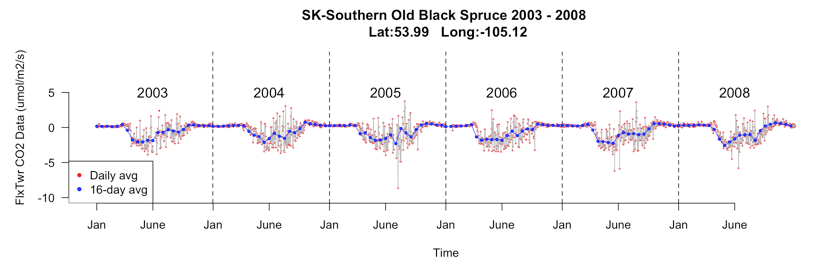
\includegraphics[width=14cm]{SOUmodis1.png}
\caption{Saskatchewan southern old black spruce CO$_2$ flux data from 2003 to 2008.}
\label{Fig:SOUmodis}
\end{figure}

SK 1975 (Young) Jack Pine site only has 3 years of CO$_2$ flux data (Figure \ref{Fig:YJPmodis}).




\begin{figure}[!ht]
\centering
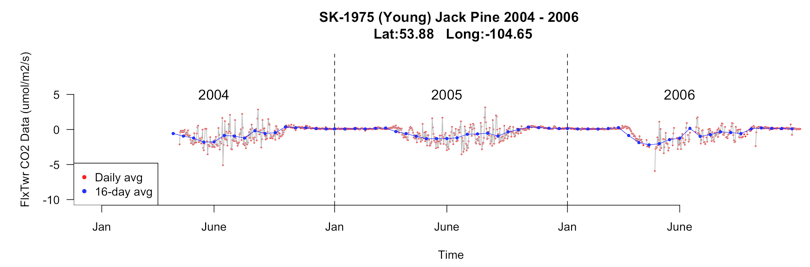
\includegraphics[width=14cm]{YJPmodis1.png}
\caption{Saskatchewan young jack pine CO$_2$ flux data from 2004 to 2006.}
\label{Fig:YJPmodis}
\end{figure}


The corresponding NDVI data for SK Old Aspen shows in Figure \ref{Fig:oapndvi}. The NDVI data for SK Old Jack Pine (Figure \ref{Fig:ojpndvi}) has a lot more variation than other sites. The NDVI data for SK Southern Old Black Spruce (Figure \ref{Fig:soundvi}) has stable performance in summer time. The NDVI of SK (Young) Jack Pine (Figure \ref{Fig:yjpndvi}) has similar behaviour as SK  Southern Old Black Spruce.



\begin{figure}[!ht]
\centering
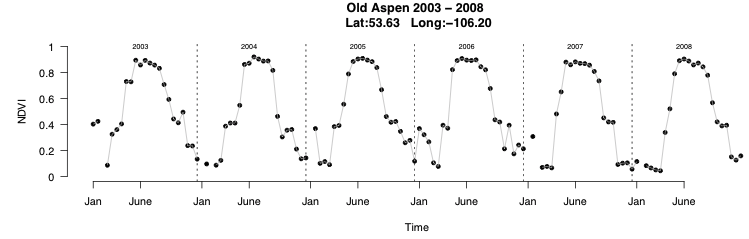
\includegraphics[width=14cm]{oapndvi.png}
\caption{Saskatchewan old aspen NDVI data from 2003 to 2008.}
\label{Fig:oapndvi}
\end{figure}



\begin{figure}[!ht]
\centering
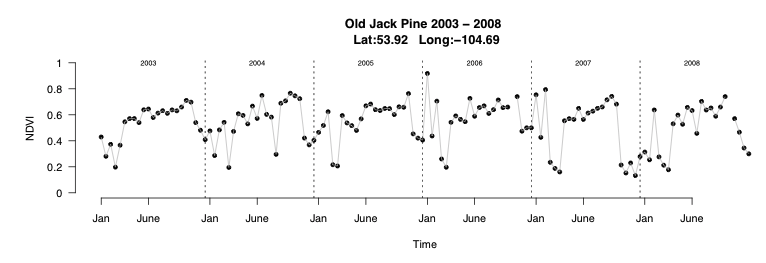
\includegraphics[width=14cm]{ojpndvi.png}
\caption{Saskatchewan old jack pine NDVI data from 2003 to 2008.}
\label{Fig:ojpndvi}
\end{figure}



\begin{figure}[!ht]
\centering
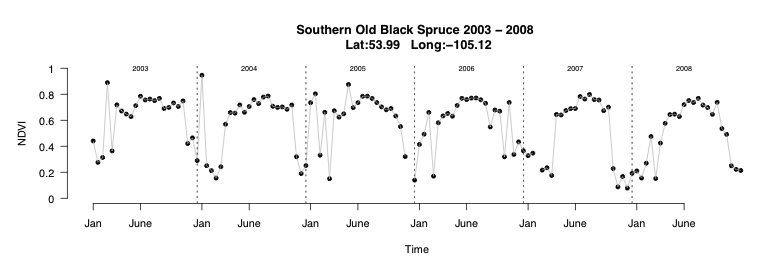
\includegraphics[width=14cm]{soundvi.png}
\caption{Saskatchewan southern old black spruce NDVI data from 2003 to 2008.}
\label{Fig:soundvi}
\end{figure}




\begin{figure}[!ht]
\centering
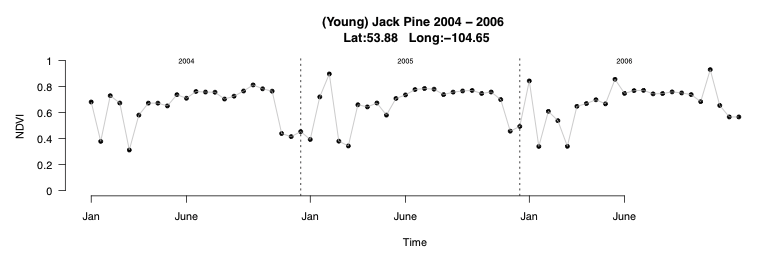
\includegraphics[width=14cm]{yjpndvi.png}
\caption{Saskatchewan young jack pine NDVI data from 2004 to 2006.}
\label{Fig:yjpndvi}
\end{figure}

\section{Methods}\label{Sec:Methods}

The class of additive models is a flexible and powerful tool. Section \ref{Sec:AddModel} describes how we applied a univariate additive model to 4 locations' CO$_2$ flux. Besides treating the CO$_2$ flux data as a single time series, we can treat each year as independent multivariate observation. Since the shape of CO$_2$ flux data is similar at each location over the year, we use functional smoothing (Section \ref{Sec:SplineSmoothing}) to capture the underlying pattern.  Except for similarity in shape, the seasonal effect is quite different year to year. Thus we make use of the idea of registration (Section \ref{Sec:Regi}). As mentioned in Section \ref{Sec:LiteratureReview}, registration can help to reduce the individual difference, and better reveal the common features. With registration, simulations can be done with less individual variability. One important element for registration is the warping function (Section \ref{Sec:Warping}). The warping function is a bridge transformation between nature/real time scale and registered time scale. We used a multivariate normal (Section \ref{Sec:MultiNormal}) to simulate new curves in the registered time scale. The next step is to transform the simulated curves back to real time scale by the inverse warping function for further study.  To simulate random warping functions, the Dirichlet regression (Section \ref{Sec:DiriReg}) is applied, and simulated values are drawn from the fitted model.


\subsection{Additive Model}\label{Sec:AddModel}

A generalized additive model (Hastie and Tibshirani, 1986, 1990) is a generalized linear model with a linear predictor involving a sum of smooth functions of covariates. It is known as GAM. 

To fit a univariate additive model, flux tower data at each of the 4 locations was used as the dependent variable,  while time (solar days), species of plants, and NDVI data are the independent variables used in the model.  Each of the locations has been modelled in the following way.


\begin{equation}
\textrm{Flux} \sim f_1\textrm{(Time)} + \textrm{Species}  + f_2\textrm{(Time,Species)} + \textrm{NDVI},\label{Eq:AddMod}
\end{equation}
where functions $f_k$  $(k=1,2)$ are smooth functions of covariates; Time is every 16 day staring at the first day of each year; Species has 4 levels, old aspen, old jack pine, old black spruce, and young jack pine; (Time,Species) is the interaction between Time and Species; NDVI is a numeric vector. $f_1(\textrm{Time})$ is the average of CO$_2$ flux by the change of $\textrm{Time}$, and $f_2\textrm{(Time,Species)}$ represents the departures for specific species. Throughout this section, we use $f$ as a generic function, which will become clear in the context.


One downside of this approach is that the meaning of estimated coefficients is not straightforward. The residuals of the fitted model are shown in Figure \ref{Fig:GAM}. To better view the residuals, we plot the residuals at each location in Figure \ref{Fig:EachRes} with the corresponding QQ plot. Figure \ref{Fig:EachRes} shows that the residuals are not follow normal distribution, and summer has more variation than winter. Assuming the data over years has the same cycle is not appropriate. The phase of the underlying pattern is different. Other model fitting tools should be applied.  We used spline smoothing (Section \ref{Sec:SplineSmoothing})  and functional registration (Section \ref{Sec:Regi}) to solve this problem.

\begin{figure}[ht]
\centering
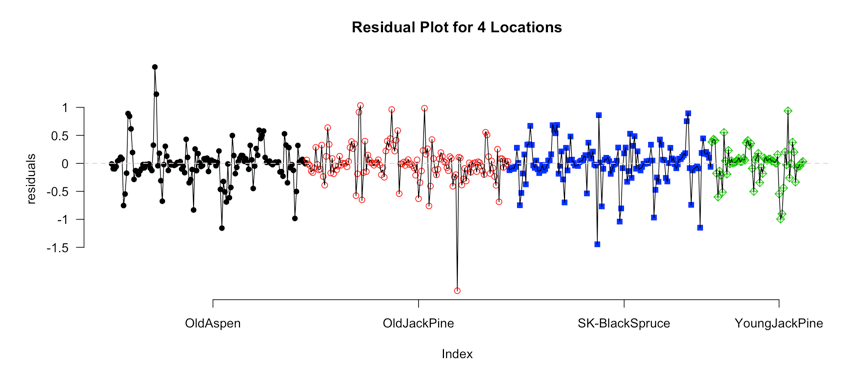
\includegraphics[width=14cm]{res3.png}
\caption{Residuals of additive model.}\label{Fig:GAM}
\end{figure}


\begin{figure}[!ht]
    \centering
    \begin{subfigure}[ht]{0.85\textwidth}
        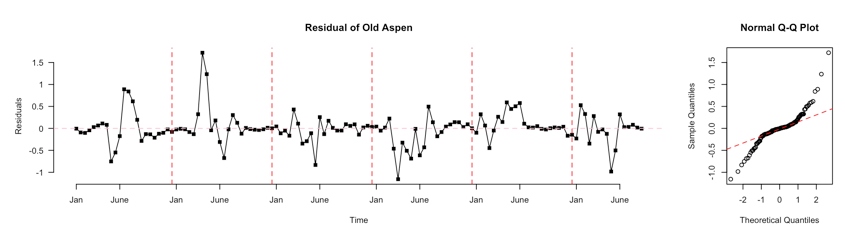
\includegraphics[width=\textwidth]{resOAP.png}
        \caption{Residuals of SK-Old Aspen location.}
    \end{subfigure}
    ~ 
    \begin{subfigure}[ht]{0.85\textwidth}
        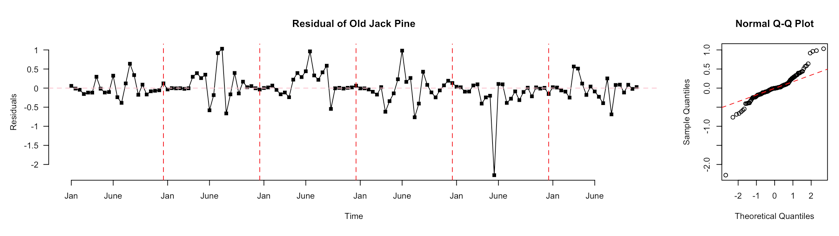
\includegraphics[width=\textwidth]{resOJP.png}
        \caption{Residuals of SK-Old Jack location.}
     \end{subfigure}
        ~ 
      \begin{subfigure}[ht]{0.85\textwidth}
        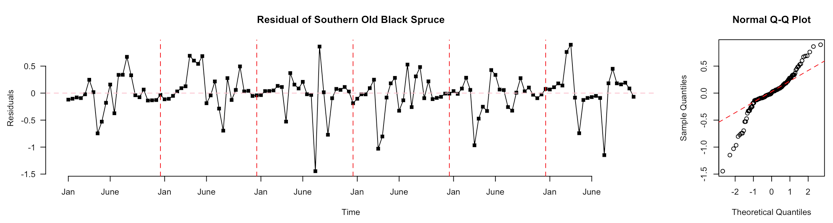
\includegraphics[width=\textwidth]{resSOU.png}
        \caption{Residuals of SK-Southern Old Black Spruce location.}
     \end{subfigure}
     ~
      \begin{subfigure}[ht]{0.85\textwidth}
        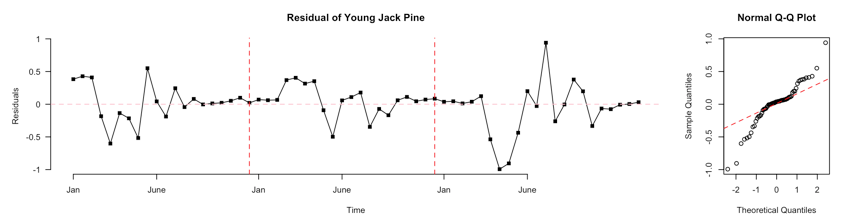
\includegraphics[width=\textwidth]{resYJP.png}
        \caption{Residuals of SK-Young Jack Pine location.}
     \end{subfigure}
    \caption{Residuals of each location of GAM and corresponding QQ plots.}\label{Fig:EachRes}
\end{figure}




\subsection{Spline Smoothing}\label{Sec:SplineSmoothing}

A $k^{th}$ order spline is a piecewise polynomial function of degree $k$, that is continuous and has continuous derivatives of orders $1,\dots,k-1$, at its knot points.

Formally, a function $\phi:\mathbb{R}\rightarrow\mathbb{R}$ is a $k^{th}$ order spline with knot points at $t_1<\dots<t_m$, if

\begin{enumerate}
\item $\phi$ is a polynomial of degree $k$ on each of the intervals $(-\infty,t_1],[t_1,t_2],\dots,[t_m,\infty)$,
\item $\phi^{(j)}$, the $j^{th}$ derivative of $\phi$, is continuous at $t_1,\dots,t_m$, for each $j=0,1,\dots,k-1$.
\end{enumerate}

The most common case considered is $k=3$, i.e. cubic splines which have continuous first and second derivatives. 

Our data have 23 data points $(t_i,y_i),\;\;i=1,\dots,23$ each year. The regression model $f(t) = E(Y|T=t)$ can be estimated by fitting a $k^{th}$ order spline with knots at some pre-specified locations $t_1,\dots,t_m$. The means considering functions of the form $f(t)=\sum_{j=1}^{m+k+1}\beta_j\phi_j(t)$, where $\beta_1,\dots,\beta_{m+k+1}$ are coefficients and $\phi_1,\dots,\phi_{m+k+1}$ are the basis functions for $k^{th}$ order splines over the knots $t_1,\dots,t_m$. The coefficients $\beta_1,\dots,\beta_{m+k+1}$ can be estimated by least squares, i.e. minimizing

\begin{equation}
\sum_{i=1}^{n}\left(y_i-f(t_i)\right)^2,
\end{equation}
and the fitted line is 

\begin{equation}
\widehat{f}(t_i) = \sum_{j=1}^{m+k+1}\widehat{\beta}_j\phi_j(t_i).
\end{equation}


The matrix form of spline regression is defined below:

\begin{equation}
\uwave{y} = \Phi\uwave{\beta}+\uwave{\epsilon},
\end{equation}
where $\uwave{y} = (y_1,y_2,\dots,y_n)^{T}$, and $\uwave{\beta} = (\beta_1,\beta_2,\dots,\beta_{m+k+1})^{T}$, and


\begin{equation}
\Phi=
  \begin{pmatrix}
  \phi_1(t_1) & \phi_2(t_1) & \cdots & \phi_{m+k+1}(t_1) \\
  \phi_1(t_2) & \phi_2(t_2) & \cdots & \phi_{m+k+1}(t_2) \\
  \vdots & \vdots & \ddots & \vdots \\
  \phi_1(t_n) & \phi_2(t_n) & \cdots & \phi_{m+k+1}(t_n)
  \end{pmatrix}.
\end{equation}

The estimated value for $\uwave{\widehat{\beta}}$  is $(\Phi^T\Phi)^{-1}\Phi^T\uwave{y}$.

We fit the data year by year for each location.
The knot points for old aspen data show in Table  1, 120, 130, 140, 170, 200, 220, 250, 260, 270, and 365 every year. 
The spline smoothing of old aspen data is shown in Figure \ref{Fig:smoothOA}. 


\begin{table}[!ht]
\caption{Knots used in old aspen data.}\label{Tab:knots}
\centering
\def\arraystretch{1.5}
\begin{tabular}{|c|ccccccccccc|}
\hline
Day of year & 1 & 120 & 130 & 140 & 170 & 200 & 220 & 250 & 260 & 270 & 365\\ \hline
Date & Jan 1 & Apr 30 & May 10 & May 20 & Jun 19 & July 19 & Aug 8 & Sep 7  & Sep 17 & Sep 27 & Dec 31\\ \hline
\end{tabular}
\end{table}


\begin{figure}[!ht]
\centering
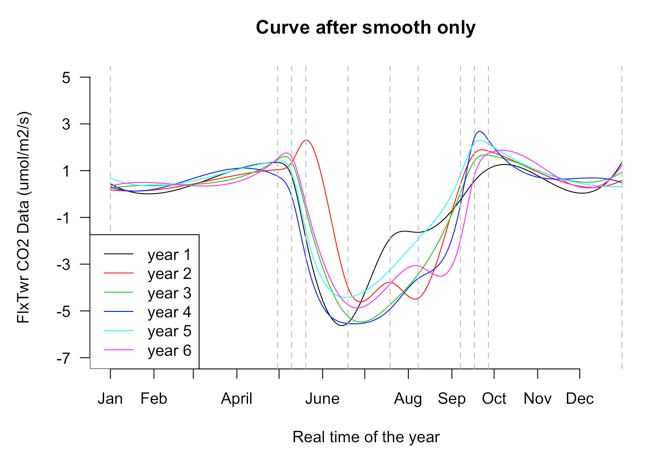
\includegraphics[width=0.58\textwidth]{Original2.png}
\caption{Spline smoothing of 6-year old aspen data. (The vertical dash lines indicate the location of knot points.)}\label{Fig:smoothOA}
\end{figure}


\subsection{Registration}\label{Sec:Regi}

The additive model (Equation \ref{Eq:AddMod}) assumes the underlying cycle is the same for every year, which may be inappropriate here.  In the flux tower data of old aspen (Figure \ref{Fig:smoothOA}), the two peaks at around May and October each year as well as the low point between the two peaks are not lined up.
We can align curves by fixing the location of a feature, such as the summer  minimum or winter maximum. 
A warping function is the connection of the original curve and the registered curve.

\subsubsection{Warping Function}\label{Sec:Warping}


We have $N$ years of data. For each year, we pick $L$ number of landmarks.
As mentioned in Section \ref{Sec:LiteratureReview}, landmarks $t_{p,v},\;p=1,\dots,N,v=1,\dots,L$  are typically maxima, minima, or zero crossings of curves. For 6-years old aspen data, we pick 3 time points, $t_{p,1},t_{p,2},t_{p,3}$,  two at the peaks (around May and October), and one at the low point (near June) every year.

We want to construct a time transformation $h(t_\textrm{regi})$. For curve at year $p$ time $t_\textrm{regi}$ the transformation is $h_p(t_\textrm{regi})$ where $1 \le t_\textrm{regi} \le 365$ such that the registered curves $f^{*}_p$ satisfy the following equations,

\begin{equation}\label{eq:warping}
f^{*}_p(t_{\textrm{regi}}) = f_p(t_{\textrm{real}}),\;\;\textrm{where }t_{\textrm{real}}=h_p(t_\textrm{regi}).
\end{equation}

The time warping function has the properties: (i) $h_p(1) = 1$, (ii) $h_p(365) = 365$, (iii) between the adjacent landmarks,  $h_p$ is linear, (iv) we also require that $h_p$ is strictly monotonic: $a < b$ implies that $h_p(a) < h_p(b)$.


\begin{figure}[!ht]
    \centering
    \begin{subfigure}[ht]{0.45\textwidth}
        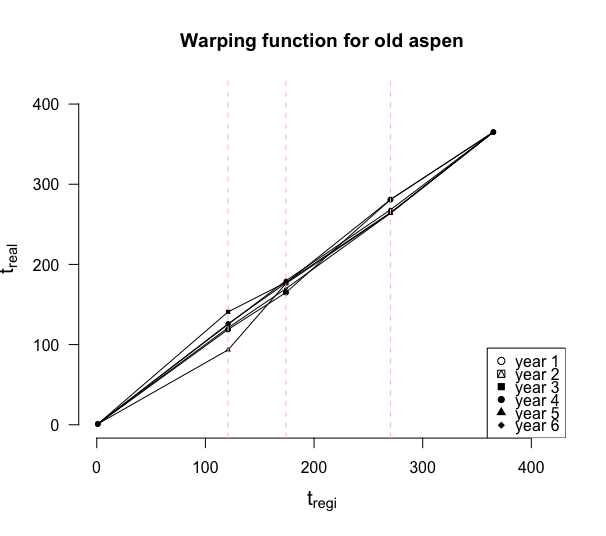
\includegraphics[width=\textwidth]{WarppingOAP4.png}
        \caption{SK-Old Aspen's warping function.}\label{Fig:warpOAP}
    \end{subfigure}
     ~
      \begin{subfigure}[ht]{0.45\textwidth}
        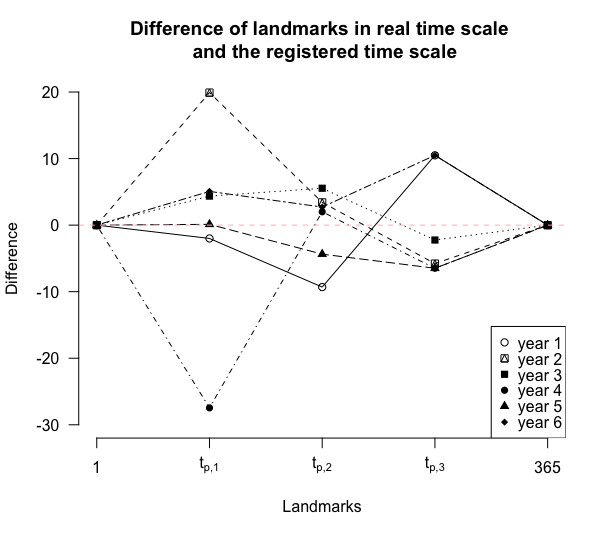
\includegraphics[width=\textwidth]{LandmarkDiff3.png}
        \caption{Landmarks of each year minus the mean landmarks.}\label{Fig:warpDiff}
     \end{subfigure}
    \caption{Old aspen's warping function and the difference of landmarks in real time scale and the registered time scale.}\label{Fig:warping}
\end{figure}

Figure \ref{Fig:warpOAP} shows the warping function for the old aspen data. 
The x axis represents time on registered time scale, and the corresponding y axis is the time on real time scale.
Over years of data, the first landmarks $t_{p,1},\;p=1,\dots,6$ on real time scale has more variation than the other two. The 3 vertical dashed lines in Figure \ref{Fig:warpOAP} show the landmarks, $t_v^{*}, v=1,\dots,3$ on registered time scale. The value of $t_v^{*}, v=1,\dots,L$ is arbitrary, we calculate them by

\begin{equation}
t_v^{*} = \frac{1}{N}\sum_{p=1}^{N} t_{p,v},\;\;v=1,\dots,L.
\end{equation}

Through the warping function, we know for a fixed year when time on registered time scale is given what's the corresponding time on real time scale should be. To better view the behaviour of landmarks, we plot the difference of landmarks in real time scale and the registered time scale in Figure \ref{Fig:warpDiff}. For year $p$ landmark $v$, we calculate the difference by

\begin{equation}
\textrm{Difference} = t_{p,i} - t_{i}^{*}.
\end{equation}



By Equation 7, we get $f^{*}_p(t_{\textrm{regi}})$ every 16 days starting from the first day of each year. We apply spline smoothing (Section \ref{Sec:SplineSmoothing}) to $f^{*}_p(t_{\textrm{regi}}),$ where $t_{\textrm{regi}}=1,17,33,\dots,353$ with the same basis when we fit the raw CO$_2$ flux data. The coefficients on the registered time scale are $\uwave{\widehat{\beta}}^{*} = (\widehat{\beta}^{*}_1,\widehat{\beta}^{*}_2,\dots,\widehat{\beta}^{*}_{m+k+1})^{T}$.  

Curves in Figure \ref{Fig:smoothOA} after registration are shown in Figure \ref{Fig:regiOA}. After registration, the peaks and valleys are lined up. Compared to Figure \ref{Fig:smoothOA}, there is less variation among lines in Figure \ref{Fig:regiOA} at any given time of the year.

\begin{figure}[!ht]
\centering
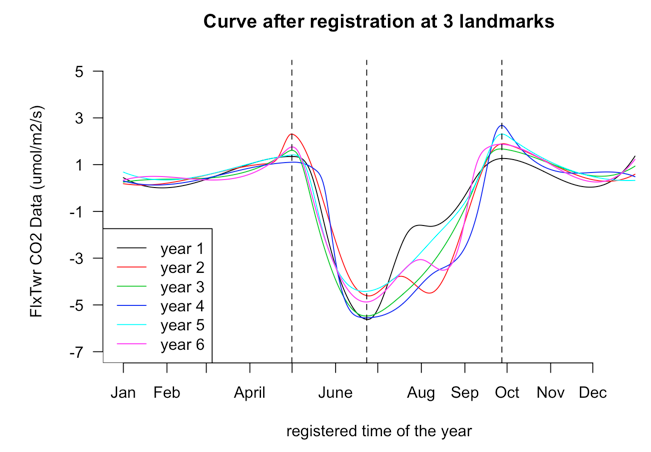
\includegraphics[width=0.6\textwidth]{Regi1.png}
\caption{Registered curves of 6-year old aspen data.}\label{Fig:regiOA}
\end{figure}


In order to simulate random CO$_2$ flux processes, there are two steps: (i) random registered curve $f^{*}_{\texttt{sim}}(t_{\textrm{regi}})$, (ii) inverse warping function. In Section \ref{Sec:MultiNormal}, we discuss how to generate random curves $f^{*}_{\texttt{sim}}(t_{\textrm{regi}})$. In Section \ref{Sec:DiriReg}, we present how to produce inverse warping function.


\subsection{A Model of the Registered Curves: Multivariate Normal}\label{Sec:MultiNormal}

We take the annual data, filtered to produce $\widehat{\beta}^{*}$ (Section \ref{Sec:Warping}). We now are looking for a distribution to model $\widehat{\beta}^{*}$. Simulated random year CO$_2$ flux data on the registered time scale can be expressed by

\begin{equation}
f^{*}_{\texttt{sim}}(t_{\textrm{regi}}) = \sum\beta^{*}_{\texttt{sim}}\phi(t_{\textrm{regi}}).\label{Eq:RegiSimu}
\end{equation}

We can model $\beta^{*}_{\texttt{sim}}$ based on $\widehat{\beta}^{*}$ using a multivariate normal distribution. Then through Equation \ref{Eq:RegiSimu} we can get the simulated curves $f^{*}_{\texttt{sim}}$ on registered time scale. 
To describe a single curve we need $m+k+1$ coefficients, a multivariate normal distribution will be used to simulate the $m+k+1$ coefficients. 

\subsubsection{Non-degenerate Case}

When the covariance matrix of $\widehat{\beta}^{*}$ is positive definite,  the distribution of multivariate normal (MVN) is given below:

\begin{equation}
f_X(x_1,\dots,x_{q}) = \frac{1}{\sqrt{(2\pi)^k|\Sigma|}}\exp\left(-\frac{1}{2}(x-\mu)'\Sigma^{-1}(x-\mu)\right),
\end{equation}
where $X$ is a real $q$-dimensional column vector, $\mu$ is a 1 by $q$ vector which is the mean of each column vector of $X$, $|\Sigma|$ is a $q$ by $q$ covariance matrix of $X$,  and $|\Sigma|$ is the determinant of $\Sigma$. 

\subsubsection{Degenerate Case}

When the covariance matrix is not full rank, $m+k+1$ by $m+k+1$ symmetric matrix $\Sigma$ of rank $d<m+k+1$. $\Sigma$ has $d$ positive eigenvalues ($\lambda_1>\lambda_2>\dots>\lambda_d>\lambda_{d+1}=0,\dots,\lambda_{m+k+1}=0$), and the $\Sigma^{-1}$ is undefined. By eigen decomposition, we have

\begin{equation}
\Sigma = EDE',
\end{equation}
where E is $m+k+1$ by $d$ matrix, and has columns which are the eigenvectors of the positive eigenvalues of the $d$ by $d$ diagonal matrix $D=diag(\lambda_1,\lambda_2,\dots,\lambda_d)$. The generalized inverse of $\Sigma$ is defined as

\begin{equation}
\Sigma^{-} = ED^{-1}E'.
\end{equation}

The p.d.f. of the singular MVN is defined over a lower dimensional subspace

\begin{equation}
f_{X}(x_1,\dots,x_{q}) = ((2\pi)^d|D|)^{-\frac{1}{2}}\exp\left\{-\frac{(x-\mu)'\Sigma^{-}(x-\mu)}{2}\right\}.
\end{equation}  


\subsection{One Simulation Method}

When covariance matrix $|\Sigma|=0$, the inverse of $\Sigma$ is not defined. To simulate MVN under this condition, we need Cholesky decomposition and linear transformation. By Cholesky decomposition, there exists a lower triangular $m+k+1$ by $m+k+1$ matrix $L$, such that 

\begin{equation}
\Sigma=LL'.
\end{equation}

Each column of $X$ is i.i.d. univariate standard normal. The number of columns of $X$ depends on the number of simulations we need. The simulated value $Y$ is

\begin{equation}
Y = \mu + LX,
\end{equation}  
where $Var(YY')= Var(LXX'L') = Var(LL')$, since $XX'$ is identity matrix. 

We apply R function mvrnorm(n$=$1,mu,Sigma) to conduct the simulation. We use the sample mean and the sample covariance to estimate $\mu$ and $\Sigma$.
We simulate 10000 CO$_2$ flux data on the registered time scale. Figure \ref{Fig:regiSimi} shows 5 simulations and 95\% point-wise prediction intervals.


\begin{figure}[!ht]
\centering
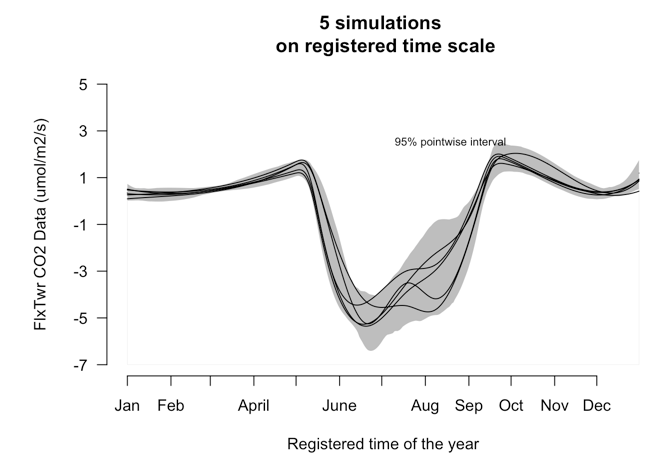
\includegraphics[width=0.6\textwidth]{regiSimi1.png}
\caption{5 simulated curves of old aspen data on the registered time scale.}\label{Fig:regiSimi}
\end{figure}


\subsection{A Model for the Inverse Warping Function: Dirichlet Regression}\label{Sec:DiriReg}

We generate $\beta^*_{\texttt{sim}}$ by MVN, which can be used to further produce $f^*_{\texttt{sim}}(t)$, the random year CO$_2$ flux data on the registered time scale. Then we need to map the the simulated curve from the registered time scale back to the real time scale.  Since we need to build a connection of registered and real time scale, we take advantage of the idea of warping function (Section \ref{Sec:Warping}).  
Compared to the previous registration which gives the landmarks on real time scale then we need to define the landmarks on registered time scale, now we know the landmarks on registered time scale, it is important to set up the landmarks  $t_{v}^{sim},\;i=1,\dots,L$ on real time scale for each simulated curve. 
  
We use two different methods to simulate the landmarks on real time scale. 
 The first model we continue using MVN.  It has the following problems,

\begin{enumerate}
\item We can't guarantee $t_1^{sim}<\dots<t_L^{sim}$.
\item Sometimes $t_{v}^{sim}$ is very close to $t_{v+1}^{sim}$.
\item We can't guarantee $1\le t_{v}^{sim}\le 365$.
\end{enumerate}

After 10000 simulation, over 95\% of the times that all the landmarks are within [0,365].
We could discard the out of range landmarks in practice.
As for the order problem, we can sort the simulated landmarks. But for the distance between landmarks, there is no easy way to solve this problem. 
Figure \ref{Fig:BadS} is an example of two landmarks generated by MVN that look too ``close'' to each other. Model other than MVN should be considered at this point.  Later in the section, we will introduce Dirichlet distribution and Dirichlet regression to overcome the problem.



\begin{figure}[!ht]
    \centering
    \begin{subfigure}[ht]{0.45\textwidth}
        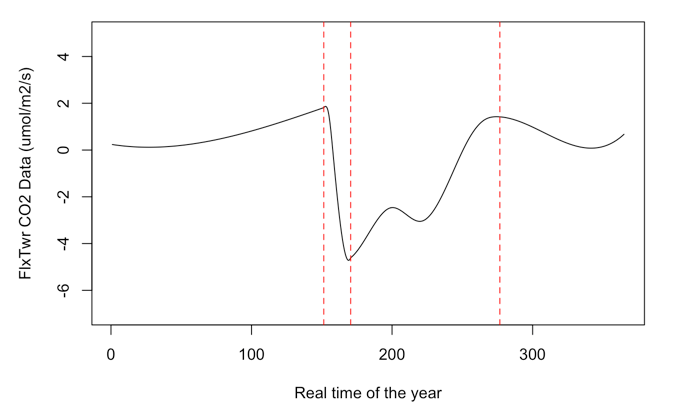
\includegraphics[width=\textwidth]{BadS2.png}
        \caption{Landmarks simulated by multivariate normal.}\label{Fig:BadS}
    \end{subfigure}
    ~ %add desired spacing between images, e. g. ~, \quad, \qquad, \hfill etc. 
      %(or a blank line to force the subfigure onto a new line)
    \begin{subfigure}[ht]{0.45\textwidth}
        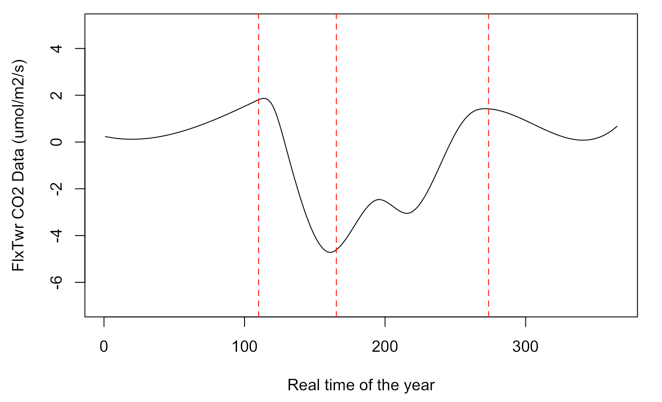
\includegraphics[width=\textwidth]{GoodS2.png}
        \caption{Landmarks simulated by Dirichlet regression.}\label{Fig:GoodS}
    \end{subfigure}
        ~ %add desired spacing between images, e. g. ~, \quad, \qquad, \hfill etc. 
      %(or a blank line to force the subfigure onto a new line)
    \caption{Landmarks generated by two methods.}\label{Fig:landCom}
\end{figure}

$L$ landmarks of year $p$ data divide $[0,365]$ to $L+1$ intervals, $[0,t_{p,1}],\;[t_{p,1},t_{p,2}],\;\dots,[t_{p,L-1},t_{p,L}]$.
The length of each interval are $l_1 = t_{p,1},\;l_2=t_{p,2}-t_{p,1},\;\dots,\;l_{L+1}=365-t_{p,L}$, and satisfy following property:

\begin{enumerate}
\item $l_1,\dots,l_{L+1}>0$
\item $\sum_{i=1}^{L+1}l_i = 365$
\end{enumerate}

Thought it is not easy to directly simulate the landmarks at the same time, there is a distribution to describe the behaviour of the intervals. It is Dirichlet distribution.  

\subsubsection{Dirichlet Distribution}


The Dirichlet distribution of order $k\ge2$ with parameters $\alpha_1,\dots,\alpha_k>0$ has a probability density function with respect to Lebesgue measure on the Euclidean space $R^{k-1}$ given by 

\begin{equation}
f(x_1,\dots,x_k;\alpha_1,\dots,\alpha_k) = \frac{1}{B(\uwave{\alpha})}\prod_{i=1}^kx_i^{\alpha_i-1},
\end{equation}
on the open $(k-1)$ dimensional simplex defined by  $x_1,\dots,x_{k-1}>0$, $x_1+\cdots+x_{k-1}<1$,  $x_k = 1- x_1-\cdots-x_{k-1}$, and zero elsewhere.

The normalizing constant is the multivariate Beta function, which can be expressed in terms of the gamma function:

\begin{equation}
B(\uwave{\alpha}) = \frac{\prod_{i=1}^k\Gamma(\alpha_i)}{\Gamma(\sum_{i=1}^k\alpha_i)},\;\;\uwave{\alpha}=(\alpha_1,\dots,\alpha_k).
\end{equation}

Compared to the properties that our $l_1,\dots,l_{L+1}$ have, if we rescale the sum of $l_1,\dots,l_{L+1}$ to 1, then the rescaled intervals exactly follow the Dirichlet distribution.


\subsubsection{Dirichlet Regression}

We assume that the $i^{th}$ year length of adjacent landmarks $y_{i.}$ where $i=1,\dots,n$ follows a Dirichlet distribution with parameter $\alpha(x_{i.})$, where $\alpha(x_{i.})=(\alpha_1(x_{i.}),\dots,\alpha_k(x_{i.}))$, and each $\alpha_l(x_{i.})$ where $l=1,\dots,k$ is a linear combination of $x_{i.}$:

\begin{equation}
\alpha_l(x_{i.}) = x_{i,1}\psi_{1,l} + x_{i,2}\psi_{2,l} +\cdots + x_{i,p}\psi_{p,l} = x_{i.}\psi_{.l}.
\end{equation}

The parameters to be estimated are $\psi=(\psi_{c,l},c=1,\dots,p,l=1,\dots,k)$, subject to the constraint $\alpha(x_{i.})>0$.


Let $x_{i.}$ be the given covariates for year $i$ where $i=1,\dots,n$, and consider the response variable $y_i=(y_{i,1},\dots,y_{i,k})$ to be a positive vector with a conditional Dirichlet distribution, $y_i|x_{i.}\sim \mathcal{D}(\alpha_1(x.),\dots,\alpha_k(x.))$. 
Assuming $y_{1.},\dots,y_{n.}$ are i.i.d. Given $\psi$, the likelihood function is

\begin{equation}
l(\psi) = \prod_{i=1}^{n}\left[\Gamma(A_i(x_{i.}))\prod_{l=1}^k\frac{y_{il}^{\alpha_l(x_{i.})-1}}{\Gamma(\alpha_l(x_{i.}))}\right],
\end{equation}
where $A_i(x_{i.})=\sum_{l=1}^k\alpha_l(x_{i.})$.

The gradients of log-likelihood is 

\begin{equation} 
\frac{\partial \log l(\psi)}{\partial\psi_{c,l}} = \sum_{i=1}^{n}\left\{[\Psi(A_i(x_{i.}))-\Psi(\alpha_l(x_{i.}))+\log y_{i,l}]x_{i,c}\right\},
\end{equation}
where $\Psi(u) = \frac{\partial log\Gamma(u)}{\partial u}$.

\medskip

Numerical methods are required to compute the maximum likelihood estimate (MLE). \citet{camargo2012estimation} discussed, and gave numerical solution of Dirichlet regression. 

Starting values and regularization policies must be carefully chosen for the optimization algorithm to converge. \citet{hijazi2009modelling} proposed a method for choosing starting values. 

\medskip

With the simulated curves $f^{*}_{sim}$ by MVN on registered time scale and the simulated landmarks by Dirichlet regression on real time scale, then we have 

\begin{equation}\label{eq:inwarping}
f^{sim}(t_{\textrm{real}}) = f^{*}_{sim}(t_{\textrm{regi}}),\;\textrm{where } t_\textrm{real}=h^{-1}(t_{\textrm{regi}}).
\end{equation}

We have $t_i^{*}$ on registered time scale, and $t_i^{sim}$ simulated by Dirichlet Regression to construct the inverse warping function.
Compared to equation \ref{eq:warping}, model in equation \ref{eq:inwarping}, transforming simulated curves from registered time scale to real time scale, uses the inverse warping function. 
Figure \ref{Fig:RealSimu} shows 10 simulated curves of old aspen data on real time scale.


\begin{figure}[!ht]
\centering
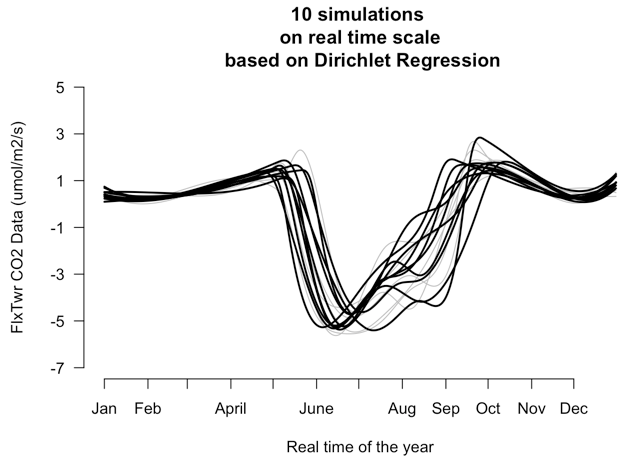
\includegraphics[width=0.6\textwidth]{RealSimu.png}
\caption{10 simulated curves of old aspen data on real time scale.}\label{Fig:RealSimu}
\end{figure}



\subsection{Kriging}\label{SubSec:Kriging}

We show how to generate random curves for one selected location in previous sections.  Currently we collect data from 4 different locations. As more and more data from different locations are going to be collected, we are interested in building a model to connect all the locations together. Kriging uses an interpolation method to connect different locations. In this section we show a brief introduction of Kriging. 

A process of interest is observed at $M$ locations $S_1,\dots,S_M$. These $n$ observations are denoted by $Z(S_1),\dots,Z(S_M)$. If the process $Z(S)$ satisfies the following two equation,

\begin{equation}
E(Z(S))=\mu
\end{equation}

\begin{equation}
Var(Z(S+h)-Z(S)) = 2\gamma(h),\;\;\forall h
\end{equation}
we say process $Z(S)$ is intrinsic stationary (IS). The difference between IS and second order stationary is presented in Appendix \ref{sec:SOSIS}.

We start by  assuming the underlying mean function has the simplest structure which is constant. More complicated case will be studied later.  Under our mean constant assumption, the process can be expressed as

\begin{equation}
Z(S) = \mu + \delta(S),
\end{equation}
where $\mu$ is the constant, and $\delta(S)$ is intrinsically stationary.

Let $S_0$ denote an unsampled location. Our goal is to find a good estimation of $Z(S_0)$, $\widehat{Z}(S_0)$, based on $Z(S_1),\dots, Z(S_M)$ (equation \ref{eq:Zso}). 

\begin{equation}\label{eq:Zso}
\widehat{Z}(S_0) = E(Z(S_0)|Z(S_1),\dots,Z(S_n))
\end{equation}

The ``good'' means $\widehat{Z}(S_0)$ minimizes $MSE(\widehat{Z}(S_0))$.

\begin{equation}\label{eq:MSE}
MSE(\widehat{Z}(S_0)) = E((\widehat{Z}(S_0)-Z(S_0))^2)
\end{equation}


Since the conditional expectation in equation \ref{eq:Zso}  is not easy to calculate, one modest way to construct $\widehat{Z}(S_0)$ is the  linear function of the observed value (equation \ref{eq:LinearCom}).

\begin{equation}\label{eq:LinearCom}
\widehat{Z}(S_0) = \sum_{i=1}^M\lambda_i Z(S_i),\,\,\textrm{where }\sum\lambda_i=1
\end{equation}

Then problem is transferred to be 

\begin{equation}
\textrm{minimize } E\left\{\left[\sum\lambda_iZ(S_i)-Z(S_0)\right]\right\}^2,\;\; \textrm{subject to}\sum\lambda_i=1.
\end{equation}


After calculation and simplification (details shown in Appendix \ref{sec:krig}), we get

\begin{equation}\label{eq:simplification}
\left[\sum\lambda_iZ(S_i) - Z(S_0)\right]^2 =\sum\lambda_i(Z(S_i)-Z(S_0))^2 - \frac{1}{2}\sum\sum\lambda_i\lambda_j(Z(S_i)-Z(S_0))^2.
\end{equation}


The variogram function $2\gamma(h)$ is defined as

\begin{equation}\label{eq:variogram}
2\gamma(h)=E((Z(S+h)-Z(S))^2),
\end{equation} 
where $\gamma(h)$ is called the semi-variogram.


We take expectation on both side of equation \ref{eq:simplification},  and combine the variogram function (equation \ref{eq:variogram}), equation \ref{eq:MSE} can be expressed as

\begin{equation}\label{eq:modiMSE}
MSE(\widehat{Z}(S_0))=E((Z(S_0)-\widehat{Z}(S_0))^2) = 2\sum\lambda_i\gamma(S_0-S_i) - \sum\sum\lambda_i\lambda_j\gamma(S_i-S_j)
\end{equation}

We use Lagrange multiplier to minimize $MSE(\widehat{Z}(S_0))$ (equation \ref{eq:modiMSE}).  

\begin{equation}\label{eq:Lagrange}
L(\lambda_1,\dots,\lambda_n) = 2\sum\lambda_i\gamma(S_0-S_i) - \sum\sum\lambda_i\lambda_j\gamma(S_i-S_j) - \theta\left(\sum\lambda_i-1\right)
\end{equation}

Differentiating $L$ (equation \ref{eq:Lagrange}) with respect to $\lambda_i$ for $i=1,\dots,M$, and $\theta$, we get

\begin{equation}
\frac{\partial L}{\partial \lambda_i} = 2\gamma(S_0-S_i) - \sum\lambda_j\gamma(S_i-S_j) - \theta,
\end{equation}
and
\begin{equation}
\frac{\partial L}{\partial \theta} =  -\sum\lambda_i +1.
\end{equation}

We set all $M+1$ derivatives equal to 0. There are $M+1$ equations and $M+1$ unknown parameters ($\lambda_i, i=1,\dots,M$ and $m$). 

\begin{equation}
\sum\lambda_j\gamma(S_i-S_j) + \frac{\theta}{2} =\gamma(S_0-S_i),\;\;i=1,\dots,M
\end{equation}
and
\begin{equation}
\sum\lambda_i = 1.
\end{equation}

If we define $\gamma_{ij}=\gamma(S_i-S_j)$, the matrix representation of the linear system  shows below

\begin{equation}\label{eq:LinearSystem}
\left[\begin{array}{*{20}c}
\gamma_{11} & \gamma_{12} & \dots & \gamma_{1M} & 1\\
\gamma_{21} & \gamma_{22} & \dots & \gamma_{2M} & 1\\
\vdots    & & & & \vdots\\
\gamma_{M1} & \gamma_{M2} & \dots & \gamma_{MM} & 1\\
1 & 1 & \dots & 1 & 0\\
\end{array}\right]  \left[\begin{array}{*{20}c}
\lambda_{1}\\
\lambda_{2}\\
\vdots\\
\lambda_{M}\\
\frac{\theta}{2}\\
\end{array}\right]=\left[\begin{array}{*{20}c}
\gamma_{01}\\
\gamma_{02}\\
\vdots\\
\gamma_{0M}\\
1\\
\end{array}\right].
\end{equation}

We can get $\widehat{\lambda}_i,\;i=1,\dots,n$, by solving equation \ref{eq:LinearSystem}.

\section{Conclusion}\label{Sec:Conclusion}

GAM is one way to model the CO$_2$ flux tower data, the detailed modelling process shows in Appendix \ref{sec:gamcode}. GAM has the following problems.

\begin{itemize}
\item The residuals neither have homogeneous variance nor are normally distributed.
\item The model interpretation is not straightforward.
\item The behaviour of seasonal dynamics, such as the start of spring and the end of fall, remains unclear. 
\end{itemize}

The steps of the other method to model the CO$_2$ flux tower data is shown in Table \ref{Tab:ModelStep}. The step 1 has already been used in multiple fields of researches.  For those researches, after registration,  the next step usually is using fPCA or other dimension reduction tools to find the main source of variation. In our case,  to understand how the annual CO$_2$ flux data behaves on real time scale is the most important thing, because on registered time scale there isn't much information of phenology, such as when spring starts and when fall ends.
We propose Step 2 and Step 3 to achieve our goal. We name Step 3 the FDA registration model. To capture the behaviour of a whole curve is not an easy task. With FDA registration model other steps, for a specific location, we can picture the behaviour of CO$_2$ flux data. 

\begin{table}[!h]
\caption{Modelling steps}\label{Tab:ModelStep}
\centering
\def\arraystretch{1.5}
\begin{tabular}{cccc}
\hline
\textbf{Steps} & & \textbf{Warping} & \textbf{Landmarks}\\
\hline 
 1 & $f^{*}_p(t_{\textrm{regi}}) = f_p(t_{\textrm{real}})$ & $t_{\textrm{real}}=h_p(t_{\textrm{regi}})$ &  $t_i^{*}=\frac{1}{N}\sum_{p=1}^Nt_{p,i}$ \\
 2 & $f^{*}_p(t_{\textrm{regi}}) \xrightarrow{MVN} f^{*}_{sim}(t_{\textrm{regi}}) $ &  & \\
 3 & $f^{sim}(t_{\textrm{real}}) = f^{*}_{sim}(t_{\textrm{regi}})$ & $t_\textrm{real}=h^{-1}(t_{\textrm{regi}})$ & $\;\;t_i^{sim}$ $\sim$ Dirichlet Regression \\
\hline
\end{tabular}
\end{table}



\section{Future Work}\label{Sec:FutureWork}


The study performed in this proposal provides basis for future research in several aspects. These aspects include:

\begin{enumerate}

\item Since the coefficients estimated by OLS follow MVN distribution, we suspect that $\widehat{\beta}^{*}$ follow asymptotic MVN distribution. In Section \ref{Sec:MultiNormal}, we used MVN without further illustration to generate coefficients $\beta^{*}_{sim}$  from $\widehat{\beta}^{*}$ under the registered time scale. We are going to detect the distribution of $\widehat{\beta}^{*}$, and gather more statistical support to make our steps more convincing. 

\item In Section \ref{Sec:DiriReg}, we applied FDA registration model (equation \ref{eq:inwarping}) to the simulated curves under registered time scale. We plan to study the distribution of our predictions, and make inference including giving specific expression of the overall prediction band. Besides, we will apply goodness of fit test to check the compatibility of the sample with our proposed probability distribution function.

\item Spatio-temporal aspect should also be studied. With respect to CO$_2$ flux data, we will consider embedding MVN and FDA registration with additional information, such as latitude, longitude, and species.  The GLM structure incorporates well with all the information. Another spatio-temporal model commonly used is Kriging.

\item We will also analyze the structure of NDVI data, and link it to CO$_2$ flux data in order to predict CO$_2$ flux data at location without towers.

\item We will apply the whole analysis to a wider range of CO$_2$ flux data.  AmeriFlux networks offers a great planform. We are going to collect CO$_2$ flux data from the sites in Figure \ref{Fig:AllSites}. More information of those sites can be found at the official website - \MYhref[brown]{http://ameriflux.lbl.gov/sites/site-list-and-pages/}{AmeriFlux Site List}.

\end{enumerate}


\begin{figure}[!ht]
\centering
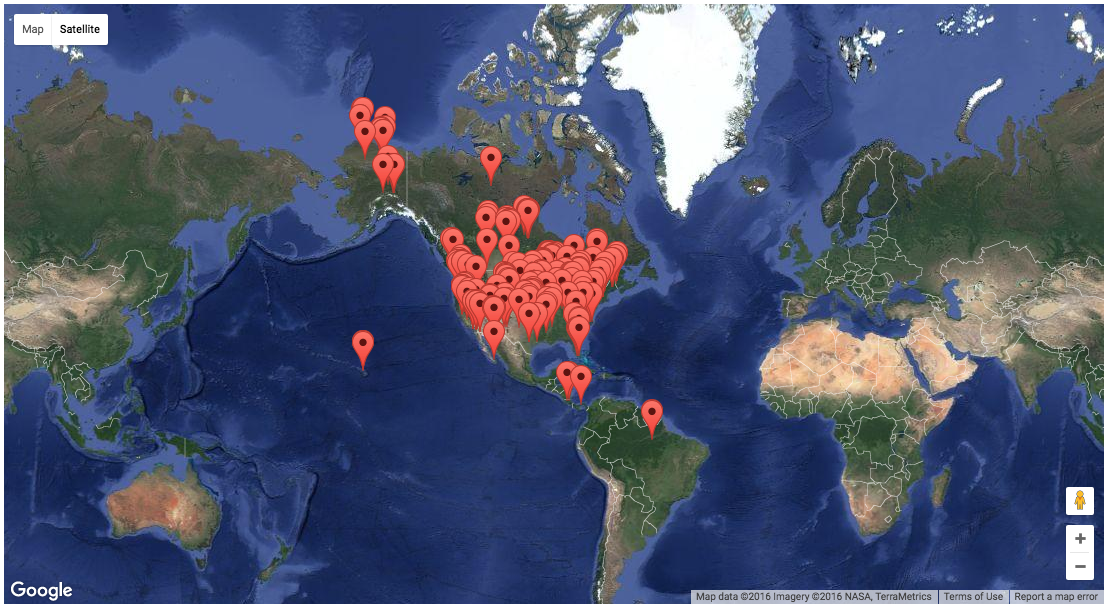
\includegraphics[width=14cm]{AllSites.png}
\caption{All Ameriflux sites.}
\label{Fig:AllSites}
\end{figure}


\clearpage


\begin{appendices}

\section{Selected Notations}

\begin{table}[!ht]
\caption{Selected notations.}\label{Tab:all_symbols}
\centering
\def\arraystretch{1.5}
\begin{tabular}{cc}
\textbf{Symbols} & \textbf{Meaning} \\
\hline\hline
$F$ & vertical fluxes \\
$\rho_a$ & air density\\
$\omega$  & vertical wind speed\\ 
$s$ & mixing ratio\\
\hline \hline
$N$ & number of years of data\\
$n$ & number of observations each year \\
$m$ & number of knot points\\
$t_i$ & interior knot points $i = 1,2,\dots,m$ \\ 
$\phi$ & spline with degree $k$ \\
$\phi^{(j)}$ & the $j^{th}$ derivative of $\phi$ \\
$L$ & length of landmarks\\ 
\hline
$\beta$ ($\widehat{\beta}$) & (fitted) coefficient of raw data on real time scale\\
$\beta^*$ ($\widehat{\beta}^*$) & (fitted) coefficient of registered smooth data on registered time scale\\
$\beta^*_{sim}$ ($\widehat{\beta}^*_{sim}$) & (fitted) coefficient of simulated registered data on registered time scale\\ 
\hline
$f_p(t_{\textrm{real}})$ &  smooth curve of year $p$ raw data\\
$f^*_p(t_{\textrm{regi}})$ & registered smooth curve of year $p$ \\
$f_{sim}^*(t_{\textrm{regi}})$ & simulated registered curve\\
$f^{sim}(t_{\textrm{real}})$ & simulated curve on real time scale\\
\hline
$t_{p,v}$ & the v$^{th}$ landmark of year $p$ smoothed curve \\
$t_v^*$ & the v$^{th}$ landmark of registered curve\\
$t_v^{sim}$ & the v$^{th}$ simulated landmark on real time scale\\
\hline\hline
$M$ & number of locations\\
$S_i$ & location $i,\;i=1,\dots,M$\\
$Z(S)$ & process at location $S$ which satisfies intrinsic stationary\\ 
\hline \hline
\end{tabular}
\end{table}

\newpage

\section{Eddy covariance method to calculate vertical flux.}\label{App:EddyCov}

In turbulent flow, $\bar{\rho}_a$ is the mean air density, $\bar{\rho}_a'$ is the deviation of $\rho_a$ from the mean air density $\bar{\rho}_a$, $\bar{\omega}$ represents the mean wind speed, $\omega'$ is the deviation in vertical wind speed $\omega$ from its mean value $\bar{\omega}$, and $\bar{s}$ is the mean value of the gas concentration, $s'$ is the deviation of gas concentration from its mean  $\bar{s}$.

Vertical flux can be presented as:

\begin{equation}
F = \overline{\rho_a\omega s}
\end{equation}

By Reynolds decomposition that $\rho_a = \bar{\rho_a} + \rho_a'$, where $\rho_a' = \rho_a - \bar{\rho_a}$, $\omega = \bar{\omega} + \omega'$, where $\omega'=\omega-\bar{\omega}$, and $s = \bar{s} + s'$, where $s'=s-\bar{s}$.

\begin{equation}
F = \overline{(\bar{\rho}_a + \rho'_a)(\bar{\omega}+\omega')(\bar{s}+s')}
\end{equation}

\begin{equation}
F= \overline{(\bar{\rho}_a\bar{\omega}\bar{s}+ \bar{\rho}_a\bar{\omega}s' +\bar{\rho}_a\omega'\bar{s}+\bar{\rho}_a\omega's'+ \rho'_a\bar{\omega}\bar{s} + \rho'_a\bar{\omega}s' + \rho'_a\omega'\bar{s}+\rho'_a\omega's')}
\end{equation}

Since the averaged deviation is zero, i.e. $\bar{\rho}'_a = \bar{\omega}' = \bar{s}'=0$ the above equation is simplified as:

\begin{equation}
F= \overline{(\bar{\rho}_a\bar{\omega}\bar{s}
+\bar{\rho}_a\omega's'
+ \rho'_a\bar{\omega}s' 
+ \rho'_a\omega'\bar{s}
+\rho'_a\omega's')}
\end{equation}

Then important assumption is make for conventional eddy covariance, which is density fluctuations are assumed negligible, i.e. $\rho'_a=0$:

\begin{equation}
F = \overline{(\bar{\rho}_a\bar{\omega}\bar{s}+\bar{\rho}_a\omega's')}
\end{equation}

Then another important assumption is made - mean vertical flow is assumed negligible for horizontal homogeneous terrain, i.e.$\bar{\omega}=0$ :

\begin{equation}
F = \overline{(\bar{\rho}_a\omega's')} = \bar{\rho}_a\overline{\omega's'}
\end{equation}

\textbf{In statistical language:}

3 random variables $\rho_a$, $\omega$ and $s$, where $\rho_a = E(\rho_a) + \epsilon_{\rho_a}$, $\omega = E(\omega)+\epsilon_{\omega}$, and $s = E(s) +\epsilon_s$.

Assumptions are $\epsilon_{\rho_a} =E(\omega)=E(\epsilon_\omega)=E(\epsilon_s)= 0$.

\begin{equation}
F = E(\rho_a\omega s)
\end{equation}

\begin{equation}
F = E[(E(\rho_a) + \epsilon_{\rho_a})(E(\omega)+\epsilon_\omega)(E(s)+\epsilon_s)]
\end{equation}

By our assumptions, the equation can be simplified as follows:

\begin{equation}
F = E[E(\rho_a)\epsilon_\omega(E(s)+\epsilon_s)]
\end{equation}

\begin{equation}
F = E[E(\rho_a)\epsilon_\omega E(s)] + E(E(\rho_a)\epsilon_\omega\epsilon_s)
\end{equation}


\begin{equation}
F = E(\rho_a)E(\epsilon_\omega)E(s) + E(E(\rho_a)\epsilon_\omega\epsilon_s)
\end{equation}

\begin{equation}
F =  E(E(\rho_a)\epsilon_\omega\epsilon_s)
\end{equation}

\textbf{Discussion}

The ``covariance'' in eddy covariance method is different from the covariance in statistics which is shown below:

\begin{equation}
Cov(X,Y) = E[(X-E(X))(Y-E(Y))]
\end{equation}

\newpage

\section{R code of GAM model (equation \ref{Eq:AddMod})}\label{sec:gamcode}

\begin{knitrout}
\definecolor{shadecolor}{rgb}{0.969, 0.969, 0.969}\color{fgcolor}\begin{kframe}
\begin{alltt}
\hlkwd{library}\hlstd{(mgcv)}
\end{alltt}


{\ttfamily\noindent\itshape\color{messagecolor}{\#\# Loading required package: nlme}}

{\ttfamily\noindent\itshape\color{messagecolor}{\#\# This is mgcv 1.8-13. For overview type 'help("{}mgcv-package"{})'.}}\begin{alltt}
\hlstd{Res.Var} \hlkwb{<-} \hlkwa{function}\hlstd{(}\hlkwc{flux.data}\hlstd{,}\hlkwc{NDVI.data}\hlstd{,}\hlkwc{n.year}\hlstd{)\{}
        \hlstd{NDVI} \hlkwb{<-} \hlstd{NDVI.data}
        \hlstd{Indi0} \hlkwb{<-} \hlkwd{c}\hlstd{(}\hlkwd{rep}\hlstd{(}\hlstr{"W"}\hlstd{,}\hlnum{5}\hlstd{),}\hlkwd{rep}\hlstd{(}\hlstr{"S"}\hlstd{,}\hlnum{15}\hlstd{),}\hlkwd{rep}\hlstd{(}\hlstr{"W"}\hlstd{,}\hlnum{3}\hlstd{))}
        \hlstd{Indi} \hlkwb{<-} \hlkwd{rep}\hlstd{(Indi0, n.year)}
        \hlstd{Time} \hlkwb{<-} \hlkwd{rep}\hlstd{(}\hlkwd{seq}\hlstd{(}\hlnum{1}\hlstd{,}\hlnum{366}\hlstd{,}\hlkwc{by}\hlstd{=}\hlnum{16}\hlstd{),n.year)} \hlcom{## here the time represent day	}
        \hlstd{mod} \hlkwb{<-} \hlkwd{gam}\hlstd{(flux.data} \hlopt{~} \hlkwd{s}\hlstd{(Time,} \hlkwc{bs}\hlstd{=}\hlstr{"cc"}\hlstd{,} \hlkwc{k}\hlstd{=}\hlnum{12}\hlstd{)} \hlopt{+} \hlstd{NDVI} \hlopt{+} \hlstd{Indi)}
        \hlkwd{var}\hlstd{(}\hlkwd{residuals}\hlstd{(mod))}
\hlstd{\}}

\hlstd{OldAspen_var} \hlkwb{<-} \hlkwd{Res.Var}\hlstd{(OldAspen_16day,OldAspen_NDVI,}\hlnum{6}\hlstd{)}
\hlstd{OldJackPine_var} \hlkwb{<-} \hlkwd{Res.Var}\hlstd{(OldJackPine_16day,OldJackPine_NDVI,}\hlnum{6}\hlstd{)}
\hlstd{Southern_var} \hlkwb{<-} \hlkwd{Res.Var}\hlstd{(Southern_16day,Southern_NDVI,}\hlnum{6}\hlstd{)}
\hlstd{YoungJackPine_var} \hlkwb{<-} \hlkwd{Res.Var}\hlstd{(YoungJackPine_16day,YoungJackPine_NDVI,}\hlnum{3}\hlstd{)}

\hlstd{FlxTwr} \hlkwb{<-} \hlkwd{c}\hlstd{(OldAspen_16day,OldJackPine_16day,Southern_16day,YoungJackPine_16day)}
\hlstd{ndvi} \hlkwb{<-} \hlkwd{c}\hlstd{(OldAspen_NDVI,OldJackPine_NDVI,Southern_NDVI,YoungJackPine_NDVI)}
\hlstd{time} \hlkwb{<-} \hlkwd{rep}\hlstd{(}\hlkwd{seq}\hlstd{(}\hlnum{1}\hlstd{,}\hlnum{365}\hlstd{,}\hlkwc{by}\hlstd{=}\hlnum{16}\hlstd{),}\hlnum{21}\hlstd{)}
\hlstd{Indi0} \hlkwb{<-} \hlkwd{c}\hlstd{(}\hlkwd{rep}\hlstd{(}\hlstr{"W"}\hlstd{,}\hlnum{5}\hlstd{),}\hlkwd{rep}\hlstd{(}\hlstr{"S"}\hlstd{,}\hlnum{15}\hlstd{),}\hlkwd{rep}\hlstd{(}\hlstr{"W"}\hlstd{,}\hlnum{3}\hlstd{)); indi} \hlkwb{<-} \hlkwd{rep}\hlstd{(Indi0,}\hlnum{21}\hlstd{)}
\hlstd{spe} \hlkwb{<-}\hlkwd{c}\hlstd{(}\hlkwd{rep}\hlstd{(}\hlstr{"OldAspen"}\hlstd{,}\hlkwd{length}\hlstd{(OldAspen_NDVI)),}\hlkwd{rep}\hlstd{(}\hlstr{"OldJackPine"}\hlstd{,}\hlkwd{length}\hlstd{(OldJackPine_NDVI)),}
\hlkwd{rep}\hlstd{(}\hlstr{"BlackSpr"}\hlstd{,}\hlkwd{length}\hlstd{(Southern_NDVI)),}\hlkwd{rep}\hlstd{(}\hlstr{"YoungJackPine"}\hlstd{,}\hlkwd{length}\hlstd{(YoungJackPine_NDVI)))}
\hlstd{Weight} \hlkwb{<-} \hlkwd{c}\hlstd{(}\hlkwd{rep}\hlstd{(}\hlnum{1}\hlopt{/}\hlstd{OldAspen_var,}\hlnum{138}\hlstd{),}\hlkwd{rep}\hlstd{(}\hlnum{1}\hlopt{/}\hlstd{OldJackPine_var,}\hlnum{138}\hlstd{),}\hlkwd{rep}\hlstd{(}\hlnum{1}\hlopt{/}\hlstd{Southern_var,}\hlnum{138}\hlstd{),}
\hlkwd{rep}\hlstd{(}\hlnum{1}\hlopt{/}\hlstd{YoungJackPine_var,}\hlnum{69}\hlstd{))}
\hlstd{w} \hlkwb{<-} \hlstd{Weight}\hlopt{/}\hlkwd{mean}\hlstd{(Weight)}
\hlstd{D} \hlkwb{<-} \hlkwd{data.frame}\hlstd{(}\hlkwc{Flx}\hlstd{=FlxTwr,}\hlkwc{Time}\hlstd{=time,}\hlkwc{NDVI}\hlstd{=ndvi,}\hlkwc{Spe}\hlstd{=spe,}\hlkwc{W}\hlstd{=w,}\hlkwc{Indi}\hlstd{=indi)}
\hlkwd{rownames}\hlstd{(D)} \hlkwb{<-} \hlkwd{paste0}\hlstd{(}\hlstr{"row"}\hlstd{,}\hlnum{1}\hlopt{:}\hlkwd{nrow}\hlstd{(D))}

\hlstd{Mix} \hlkwb{<-} \hlkwd{gam}\hlstd{(Flx} \hlopt{~} \hlkwd{s}\hlstd{(Time,}\hlkwc{bs}\hlstd{=}\hlstr{"cc"}\hlstd{,}\hlkwc{k}\hlstd{=}\hlnum{23}\hlstd{)}\hlopt{+}\hlkwd{s}\hlstd{(Time,}\hlkwc{bs}\hlstd{=}\hlstr{"cc"}\hlstd{,}\hlkwc{k}\hlstd{=}\hlnum{23}\hlstd{,}\hlkwc{by}\hlstd{=Spe)}\hlopt{+} \hlstd{Spe} \hlopt{+} \hlstd{NDVI,}
\hlkwc{weights} \hlstd{= W,}\hlkwc{data} \hlstd{= D)}
\end{alltt}
\end{kframe}
\end{knitrout}

\begin{knitrout}
\definecolor{shadecolor}{rgb}{0.969, 0.969, 0.969}\color{fgcolor}\begin{kframe}
\begin{alltt}
\hlkwd{summary}\hlstd{(Mix)}
\end{alltt}
\begin{verbatim}
## 
## Family: gaussian 
## Link function: identity 
## 
## Formula:
## Flx ~ s(Time, bs = "cc", k = 23) + s(Time, bs = "cc", k = 23, 
##     by = Spe) + Spe + NDVI
## 
## Parametric coefficients:
##                  Estimate Std. Error t value Pr(>|t|)    
## (Intercept)      -0.45187    0.08211  -5.503 6.42e-08 ***
## SpeOldAspen      -0.04668    0.07315  -0.638    0.524    
## SpeOldJackPine    0.22616    0.03900   5.799 1.30e-08 ***
## SpeYoungJackPine  0.01609    0.05146   0.313    0.755    
## NDVI             -0.00197    0.13546  -0.015    0.988    
## ---
## Signif. codes:  0 '***' 0.001 '**' 0.01 '*' 0.05 '.' 0.1 ' ' 1
## 
## Approximate significance of smooth terms:
##                                edf Ref.df      F  p-value    
## s(Time)                  1.418e+01     21 20.901  < 2e-16 ***
## s(Time):SpeBlackSpr      2.768e+00     21  1.133 2.91e-07 ***
## s(Time):SpeOldAspen      1.218e+01     21 26.880  < 2e-16 ***
## s(Time):SpeOldJackPine   2.009e+00     21  0.649 6.42e-05 ***
## s(Time):SpeYoungJackPine 1.148e-08     21  0.000    0.685    
## ---
## Signif. codes:  0 '***' 0.001 '**' 0.01 '*' 0.05 '.' 0.1 ' ' 1
## 
## R-sq.(adj) =  0.835   Deviance explained = 84.7%
## GCV = 0.1435  Scale est. = 0.13235   n = 465
\end{verbatim}
\end{kframe}
\end{knitrout}

\begin{knitrout}
\definecolor{shadecolor}{rgb}{0.969, 0.969, 0.969}\color{fgcolor}\begin{kframe}
\begin{alltt}
\hlkwd{par}\hlstd{(}\hlkwc{mfrow}\hlstd{=}\hlkwd{c}\hlstd{(}\hlnum{3}\hlstd{,}\hlnum{2}\hlstd{));}\hlkwd{plot}\hlstd{(Mix,}\hlkwc{residuals}\hlstd{=T,}\hlkwc{pch}\hlstd{=}\hlnum{20}\hlstd{,}\hlkwc{cex}\hlstd{=}\hlnum{0.6}\hlstd{)}
\end{alltt}
\end{kframe}
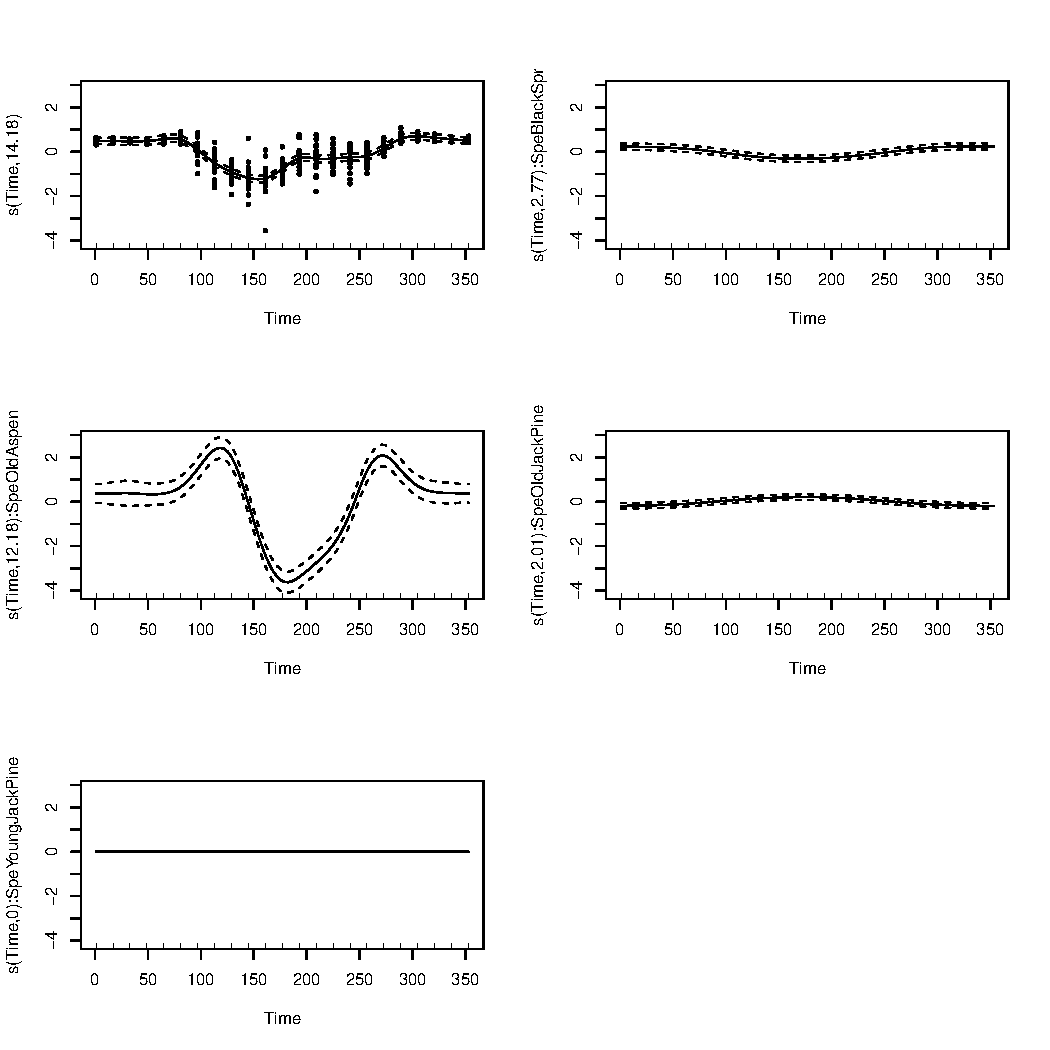
\includegraphics[width=\maxwidth]{figure/unnamed-chunk-13-1} 

\end{knitrout}

\begin{knitrout}
\definecolor{shadecolor}{rgb}{0.969, 0.969, 0.969}\color{fgcolor}\begin{kframe}
\begin{alltt}
\hlkwd{layout}\hlstd{(}\hlkwd{matrix}\hlstd{(}\hlkwd{c}\hlstd{(}\hlnum{4}\hlstd{,}\hlnum{1}\hlstd{,}\hlnum{1}\hlstd{,}\hlnum{5}\hlstd{,}\hlnum{2}\hlstd{,}\hlnum{2}\hlstd{,}\hlnum{3}\hlstd{,}\hlnum{3}\hlstd{),}\hlkwc{nrow}\hlstd{=}\hlnum{2}\hlstd{,}\hlkwc{byrow}\hlstd{=T))}
\hlkwd{qqnorm}\hlstd{(}\hlkwd{residuals}\hlstd{(Mix))}
\hlkwd{qqline}\hlstd{(}\hlkwd{residuals}\hlstd{(Mix),}\hlkwc{col}\hlstd{=}\hlnum{2}\hlstd{)}
\hlkwd{acf}\hlstd{(}\hlkwd{residuals}\hlstd{(Mix))}
\hlkwd{pacf}\hlstd{(}\hlkwd{residuals}\hlstd{(Mix))}
\end{alltt}
\end{kframe}
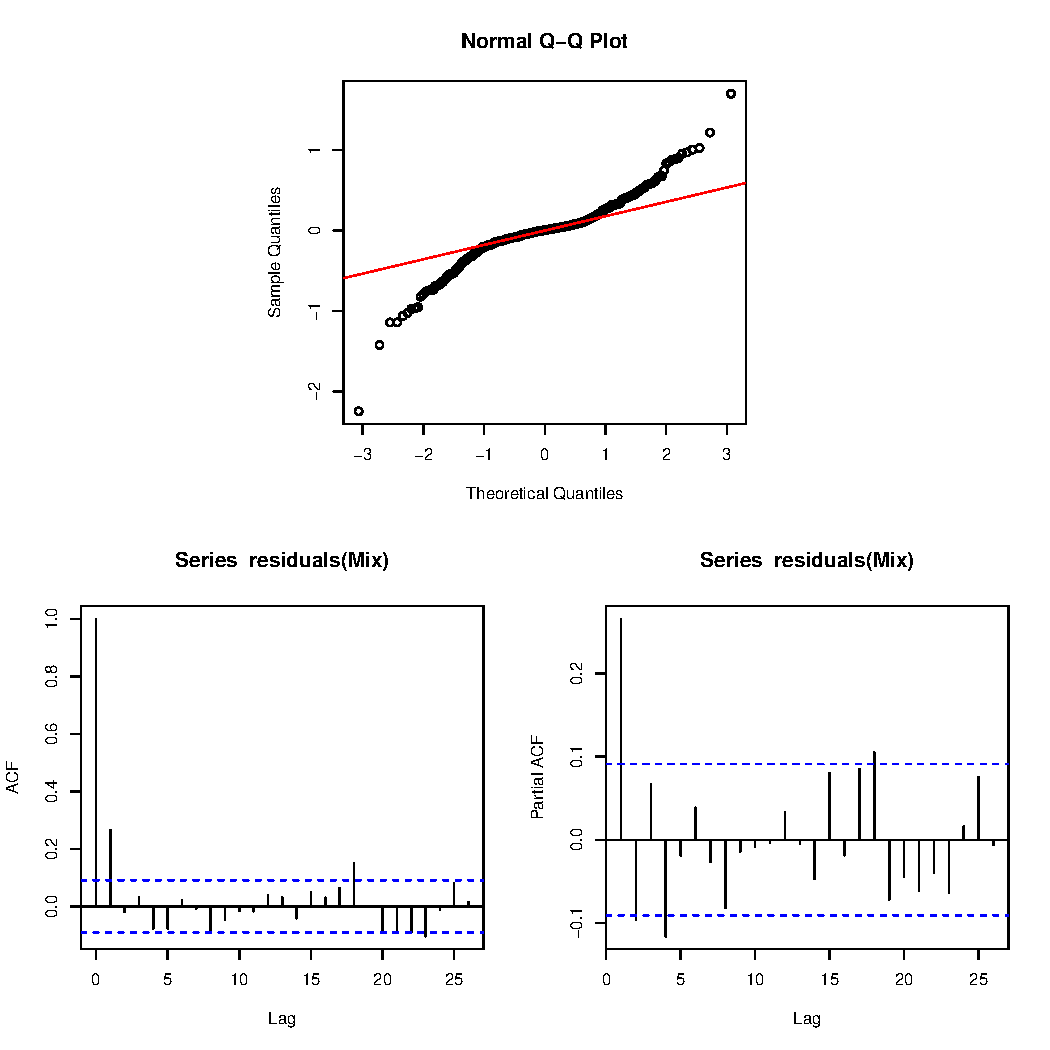
\includegraphics[width=\maxwidth]{figure/unnamed-chunk-14-1} 

\end{knitrout}


\newpage

\section{The detail of equation \ref{eq:simplification}}\label{sec:krig}

%\begin{align}
%\left[\sum\lambda_iZ(S_i) - Z(S_0)\right]^2 & =Z^2(S_0)+\left(\sum\lambda_iZ(S_i)\right)^2 - 2Z(S_0)\sum\lambda_iZ(S_i)\\
% & = Z^2(S_0) + \sum\sum\lambda_i\lambda_jZ(S_i)Z(S_j) - 2Z(S_0)\sum\lambda_iZ(S_i)\\
% & \begin{align}=[Z^2(S_0)-2\sum\lambda_iZ(S_i)Z(S_0)+\sum\lambda_iZ^2(S_i)]\\
%  + [\sum\sum\lambda_i\lambda_jZ(S_i)Z(S_j)-\sum\lambda_iZ^2(S_i)]\end{align}\\
% & \begin{align} = - \left[\frac{1}{2}\sum\lambda_j\sum\lambda_iZ^2(S_i)+\frac{1}{2}\sum\lambda_j\sum\lambda_iZ^2(S_j) - \sum\sum\lambda_i\lambda_jZ(S_i)Z(S_j)\right]\\+\left[\sum\lambda_iZ^2(S_0)-2\sum\lambda_iZ(S_i)Z(S_0)+\sum\lambda_iZ^2(S_i)\right] \end{align}\\
% & =\sum\lambda_i(Z(S_i)-Z(S_0))^2 - \frac{1}{2}\sum\sum\lambda_i\lambda_j(Z(S_i)-Z(S_0))^2
%\end{align}

\newpage

\section{Difference between second order stationary and intrinsic stationary}\label{sec:SOSIS}

\begin{itemize}
\item Second order stationary (SOS) 
\begin{enumerate}
\item \begin{equation}E(Z(S))=\mu\end{equation}
\item \begin{equation}COV(Z(S),Z(S+h))=COV(Z(0),Z(h))=C(h),\;\;\forall h\end{equation}
\end{enumerate}
\item Intrinsic stationary (IS)
\begin{enumerate}
\item \begin{equation}E(Z(S))=\mu\end{equation}
\item \begin{equation}Var(Z(S+h)-Z(S)) = 2\gamma(h),\;\;\forall h\end{equation}
\end{enumerate}
\end{itemize}

Under IS assumption:

\begin{align}
2\gamma(h) & = Var(Z(S+h)-Z(S)) \\
& = E\{[ (Z(S+h)-Z(S))-E(Z(S+h)-Z(S)) ]^2\}\\
& = E\{[Z(S+h)-Z(S)]^2\},\;\;\forall h
\end{align}

If SOS holds, 

\begin{align}
2[C(0)-C(h)] & =2[Cov(Z(S),Z(S))-Cov(Z(S+h),Z(S))]\\
& = 2[Var(Z(S))-Cov(Z(S+h),Z(S))]\\
& = 2Var(Z(S)) - 2 Cov(Z(S+h),Z(S))\\
& = Var(Z(S+h)) + Var(Z(S)) - 2 Cov(Z(S+h),Z(S))\\
& = Var(Z(S+h)-Z(S))\\
& = 2\gamma(h),\;\;\forall h,
\end{align}
which satisfies the IS assumptions too. 

Let's consider AR(1) process  $Z_i = \phi Z_{i-1}+\epsilon_i$ with $\phi=1$. That is 

\begin{equation}
Z_i = Z_{i-1}+\epsilon_i.
\end{equation}

By iteration,

\begin{equation}
Z_{i +j} = Z_i + \sum_{k=1}^j \epsilon_{i+k}.
\end{equation}

So the covariance of $Z_{i+j}$ and $Z_i$ is

\begin{equation}
Cov(Z_{i+j},Z_i) = Var(Z_i),
\end{equation}
which is a function of $i$. This doesn't satisfy SOS. However, 

\begin{align}
Var(Z_{i+j}-Z_i) & = Var(Z_i + \sum_{k=1}^j \epsilon_{i+k}-Z_i)\\
 & = Var(\sum_{k=1}^j \epsilon_{i+k})\\
 & = jVar(\epsilon_i),
\end{align}
which IS holds.

\end{appendices}


\newpage
\bibliography{fang}

\end{document}
